\chapter{Cucurrency}

\section{Cucurrency and Thread}

    Thread: very much like process, except threads share the same address space and thus
    can access the same data.


\ssc{Similarities between Processes and Threads}

    A thread has a program counter(PC), own set of registers. When switching from
    thread T1 to thread T2, a context switch must take place. There would be 
    thread control blocks (TCB) like PCB to store the state of each thread.

\ssc{Difference between Processes and Threads}

    1. The address space of threads within a single process is the same.

    2. Multi-threaded Address Spaces has different structure: one stack per thread called
    \tbi{thread-local} storage.

    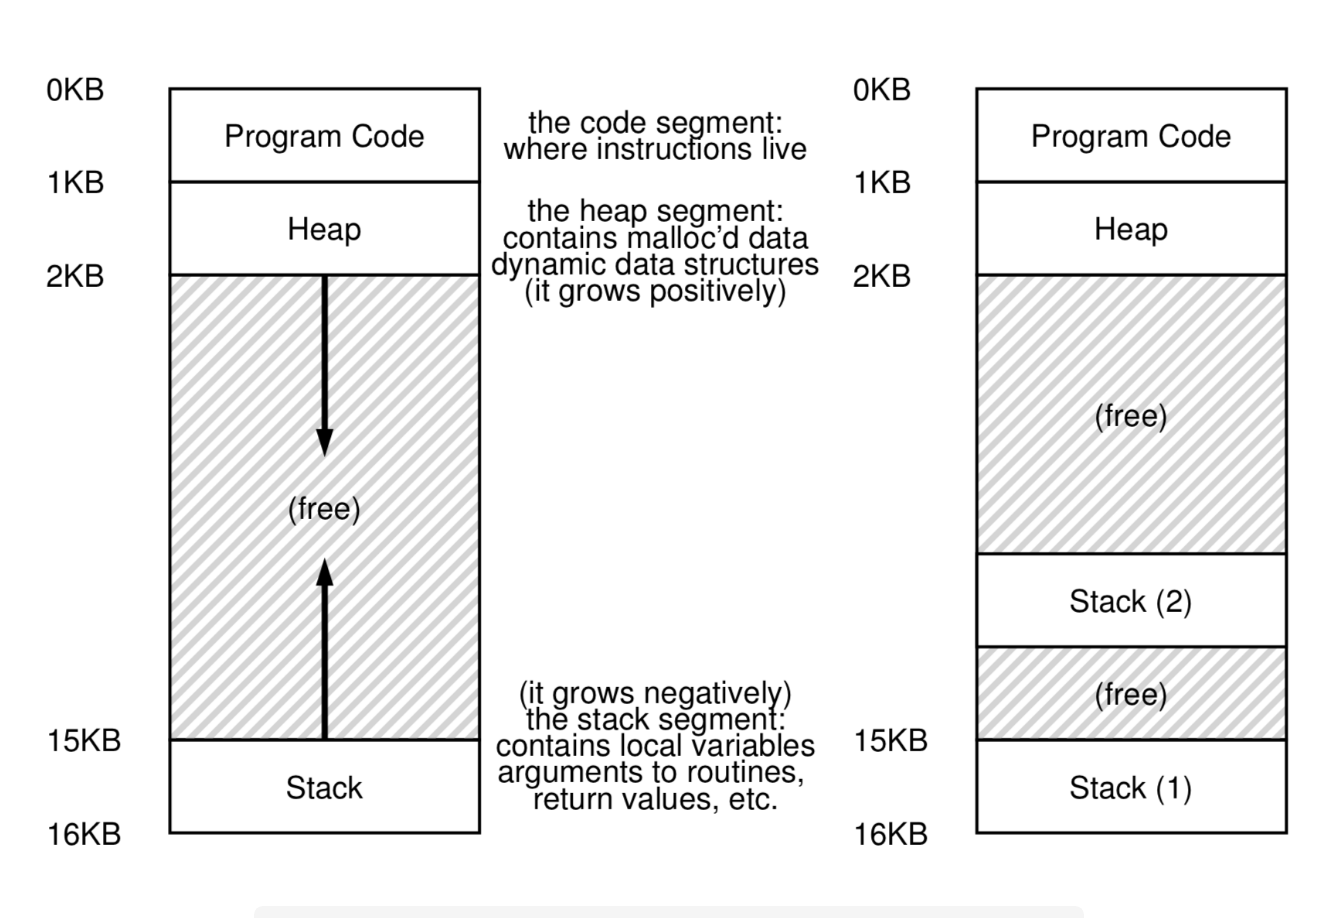
\includegraphics[width=0.65\textwidth]{chapters/Cucurrency/Cucurrency/ThreadAddressSpace.png}

\ssc{Benefit of using threads}

\sssc{Parallelism}

    Run works parallelly.

\sssc{Avoid Blocking}

    Avoid blocking program progress due to slow I/O; while one thread
    in the program waits, the CPU scheduler can switch to other ready threads.

    Threading enables overlap of I/O with other activities within a single program.

\sssc{Why not use processes instead?}

    Threads make it easy to share data, and often used to corporate with other threads
    to finish tasks.

    Processes are more sound choice for logically seperate tasks when little sharing
    of data structures in memory is needed.


\ssc{Problem with threads: Race Condition}

    \tbi{The execution sequence of threads is indeterministic}.

    Create two threads to update on the same global variable with the same function.
    
    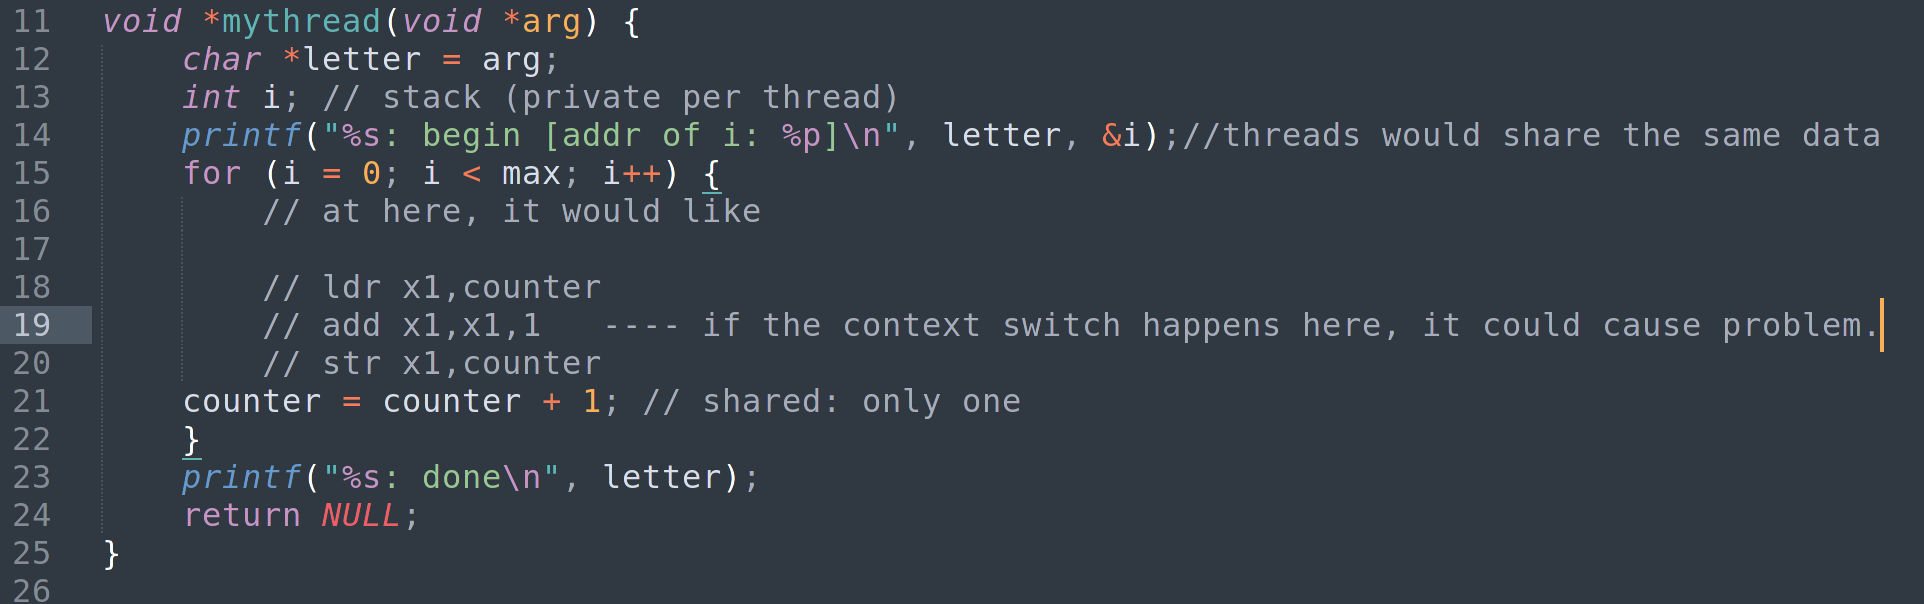
\includegraphics[width=0.75\textwidth]{chapters/Cucurrency/Cucurrency/thread_function.png}

    The problem can be:

    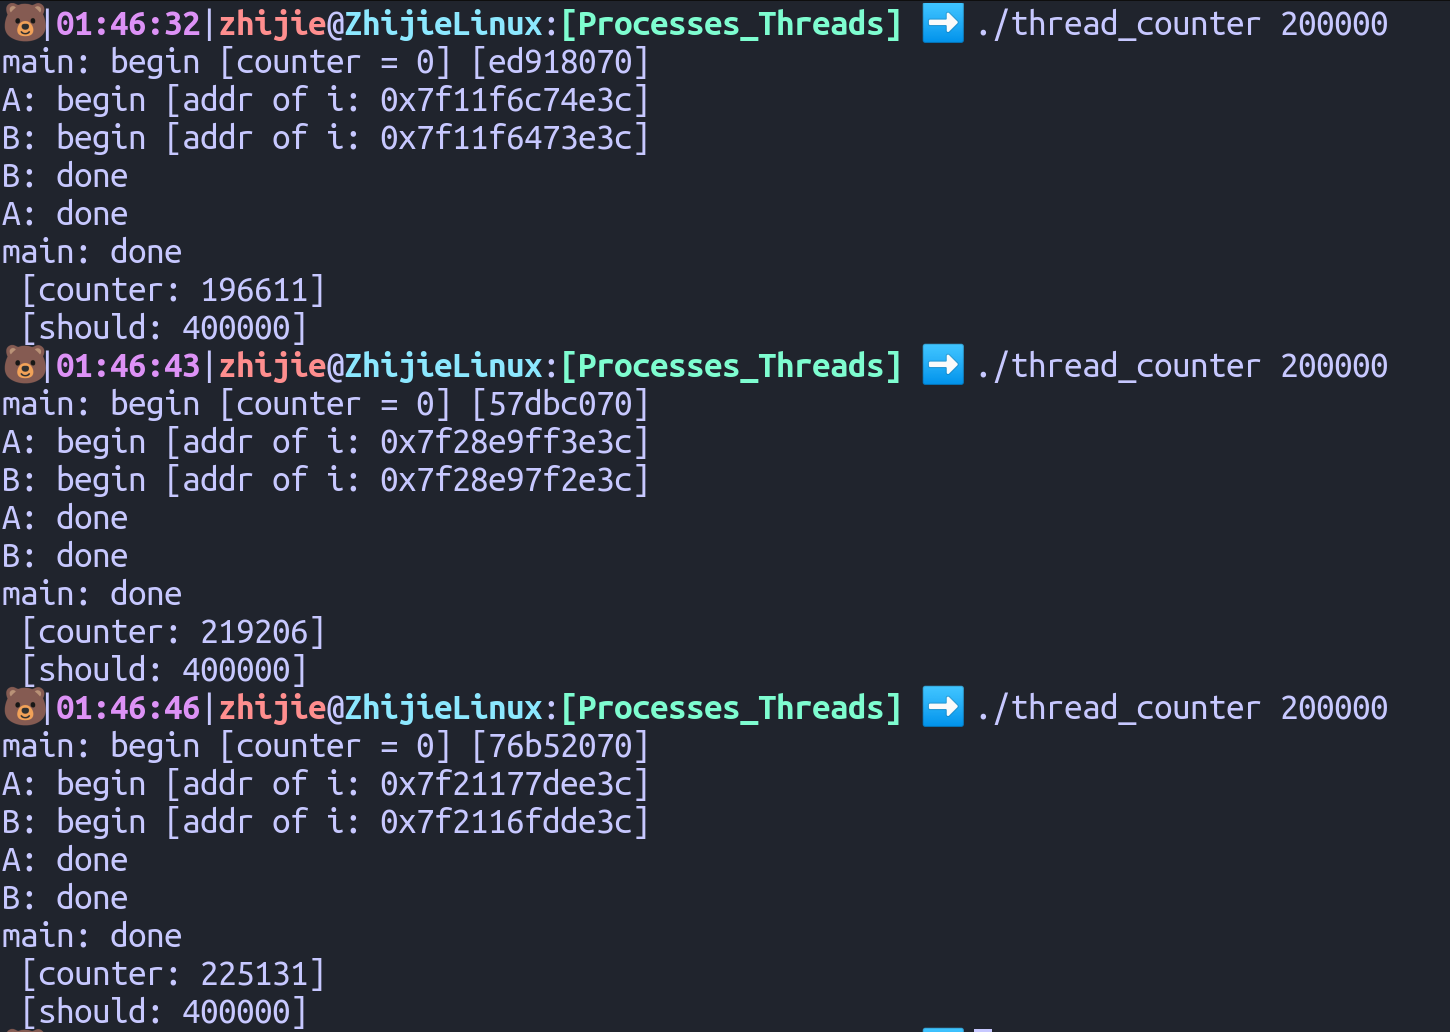
\includegraphics[width=0.7\textwidth]{chapters/Cucurrency/Cucurrency/thread_conflicts.png}


\sssc{Assembly Code}

    In ARMx8 Assembly:

    counter = counter + 1 is equivalent to 
    \begin{enumerate}
        \item ldr x1,[counter]
        \item add x1, x1, 1
        \item str x1, [counter]
    \end{enumerate}

\sssc{The work flow of causing problem}

    \begin{enumerate}
        \item Thread A loads counter into x1, say x1=50.
        \item Context switch happenes, and switch to Thread B.
        \item Now thread B loads counter into x1, x1=50.
        \item Thread B increase x1 by 1, x1=51.
        \item Thread B stores x1 back to counter, counter=51.
        \item Context switch happenes, and switch back to Thread A.
        \item Context Switch restores x1 for A,i.e, x1=50. And A won't load counter to x1 again
        \item Thread A increase x1 by 1, x1=51.
        \item Thread A stores x1 back to counter, counter=51.
        \item Thus, counter is set to 51 twice, although it should be 52 after the flow.
    \end{enumerate}

\sssc{Critical Section}

   \tbi{Critical Section}: A piece of code that accesses a shared variable, and
   must not be concurrenctly executed by more than one thread.
   
\sssc{Mutual Exclusion}

    \tbi{Mutual Exclusion:} if one thread is executing within the critical section, 
    the others will be prevented from doing so.

\sssc{Race Condition}

    Multiple threads of execution enter the critical section at roughly the same
    time; both attempt to update the shared data structure, 
    leading unexpected outcome.

\sssc{Atomicity}

    Atomic operation: grouped actions to be executed in one scheduling, i.e,
    the operation won't be interrupted.

    For example, x1 = x1 + x2 could be done in one single step with hardware support,
    instead of load, add, and store.

    It is desired to support atomicity for critical sections.   



\ssc{Thread API}

\sssc{Lock}
     
    In POSIX library, a lock needs to be initialized

    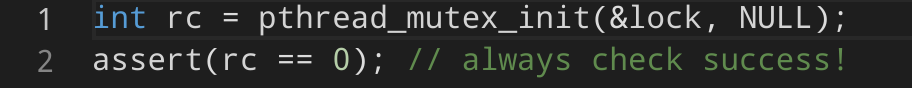
\includegraphics[width=0.6\textwidth]{chapters/Cucurrency/Cucurrency/init_lock.png}

    Also, a thread can acquire a lock, and release a lock.

    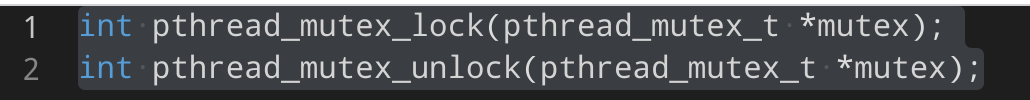
\includegraphics[width=0.6\textwidth]{chapters/Cucurrency/Cucurrency/lock_unlock.png}


\sssc{Condition Variable}

    Condition variables are useful when some kind of signaling must take place
    between threads if one thread is waiting for another to do something before it 
    continues.

    
\includegraphics[width=0.6\textwidth]{chapters/Cucurrency/Cucurrency/condtion_wait_signal.png}

    A thread must hold a lock to call either wait() or signal(). 
    $pthread_cond_wait()$, puts the calling thread to sleep.
    $pthread_cond_signal()$ awakes the waiting thread.

    The reason that $pthread_cond_wait()$ takes two parameter is because
    it needs to specify which thread to give the lock to. When $pthread_cond_wait()$
    the calling thread release the lock and pass it to another thread.

\ssc{Locks and Building one}

\sssc{Basic}

    Lock is used around the critical section. It is a global variable that either 
    available or acquired and exactly one thread can hold it at a time.

    \tbi{mutex} in POSIX means \tbi{mutual exclusion} between threads.

\sssc{Evaluating Locks}

    Basic criteria:
    \begin{enumerate}
        \item Mutual exclusion: A lock must provide mutual exclusion, i.e, the lock
        should preventing multiple threads from entering a critical section.
        \item Fairness: Prevent starving a lock.
        \item Performance: How many overhead would be added to use the lock.
    \end{enumerate}

\sssc{Lock by Controlling Interrupts}

    One of the earliest implementation of lock is disable interrupts.

    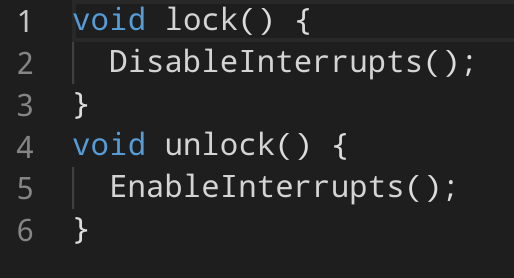
\includegraphics[width=0.6\textwidth]{chapters/Cucurrency/Cucurrency/earliest_lock.png}

    This approach works since it assumes mutual exclusion, and it is very simple.

    However, it has flaws:
    \begin{enumerate}
        \item Priviledged action: malicious process would disable the interrupts and
        never enable interrupts again.
        \item Interrupts would get lost: for example, I/O interrupts would get lost 
        and some processes which are waiting on those interrupts cannot move forward.
        \item Inefficient approach: It is very costly to enable/disable interrupts.
        \item No support for multiprocessors.
    \end{enumerate}

\sssc{A Fail Attempt: Using a Flag}

    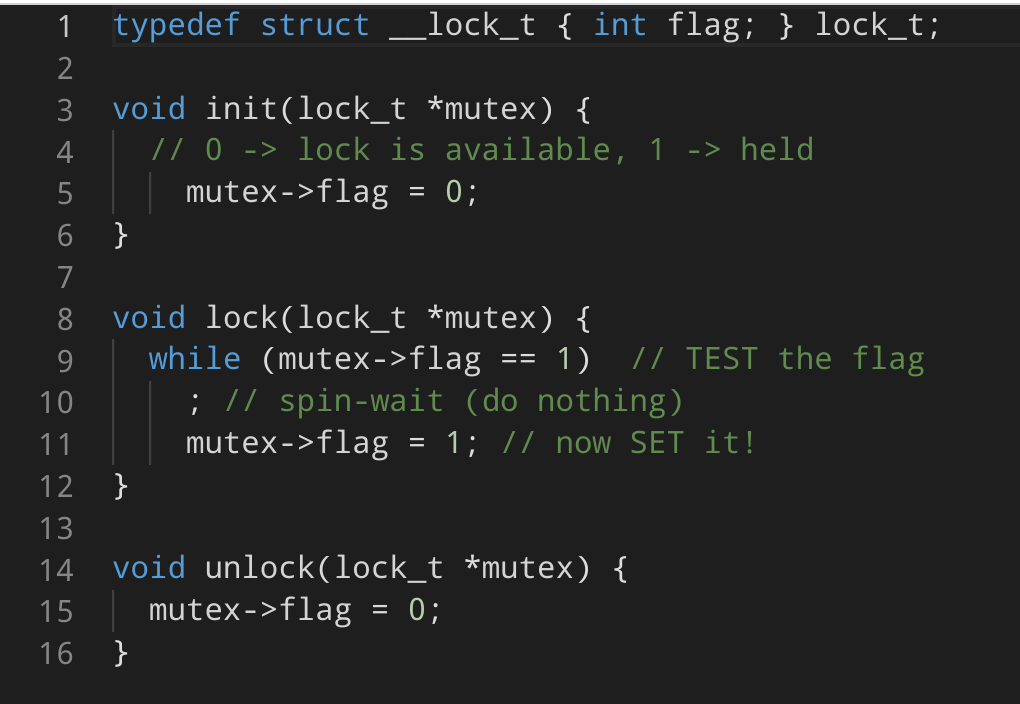
\includegraphics[width=0.6\textwidth]{chapters/Cucurrency/Cucurrency/lock_by_flag.png}

    \tbi{Correctness Problem}: Interleaving would give more locks than just one.

    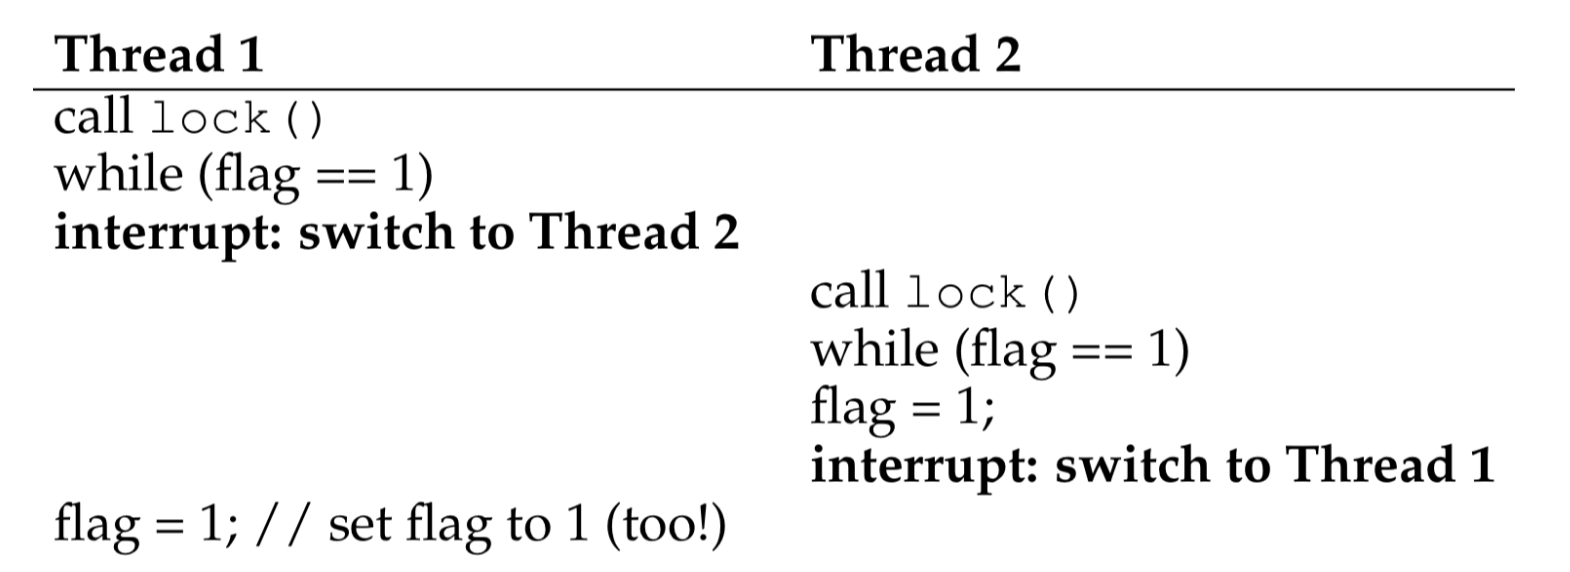
\includegraphics[width=0.6\textwidth]{chapters/Cucurrency/Cucurrency/Interleaving_problem.png}

    \tbi{Performance Problem}: While loops is valid instruction that would use CPU,
    it is very likely a thread which acquiring the lock spents its timeslot to 
    loop. This behavior is called \tbi{busy-waiting} or \tbi{spin-waiting}.

\sssc{Test-and-Set}

    \tbi{Test-and-Set} is atomic instruction supported by the hardware. It 
    both gets and sets the value in a register/address. 

    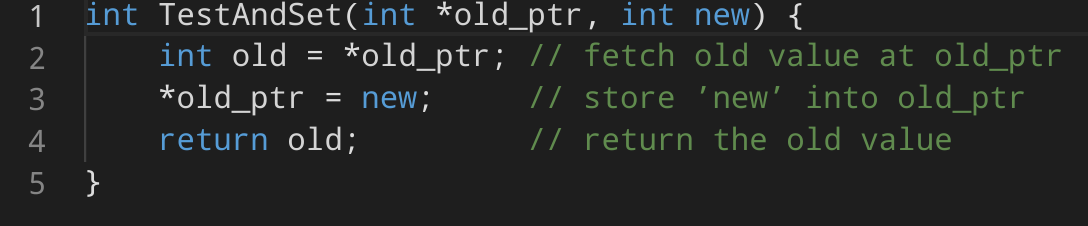
\includegraphics[width=0.6\textwidth]{chapters/Cucurrency/Cucurrency/test_and_set.png}

    With \tbi{Test-and-Set}, we can build a correct lock.

    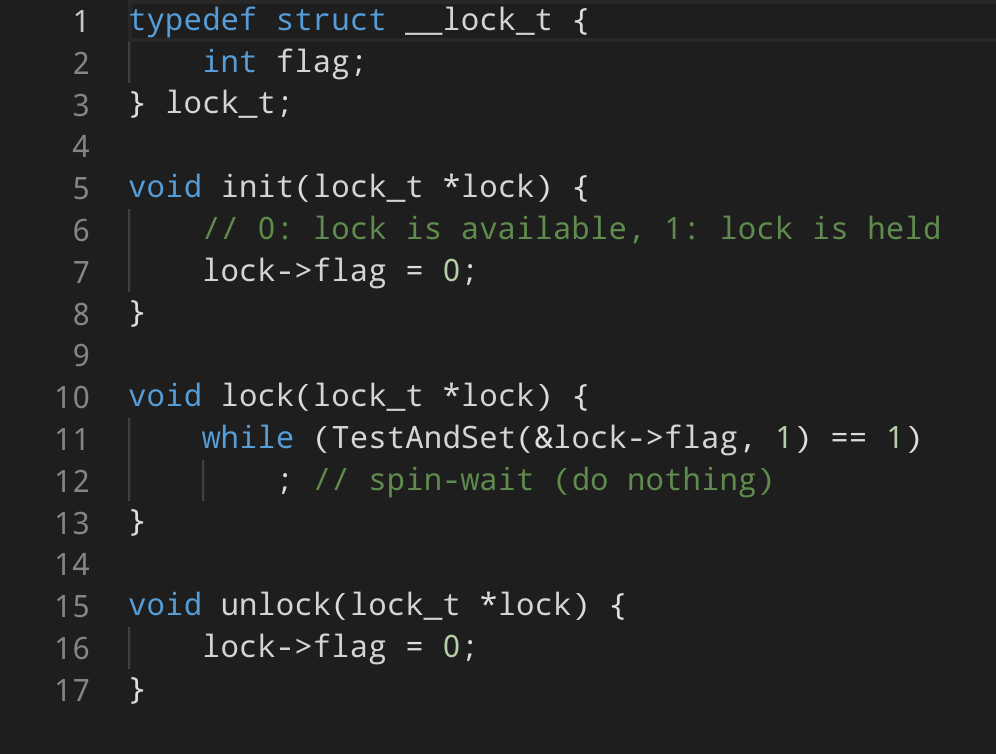
\includegraphics[width=0.7\textwidth]{chapters/Cucurrency/Cucurrency/spin_locks_test_set.png}

    However, the Test-and-Set approach doesn't guarantee
    \begin{enumerate}
        \item Fairness: There is no intelligence invoked to provide fairness.
        \item Performance: It is painful on a single CPU. Acceptable on multiple CPUs,
        because the CPU scheduler would switch the waiting thread out after its timeslot.
    \end{enumerate}

\sssc{Compare-And-Swap}

    \tbi{Compare-And-Swap}: Test whether the value equals; is so, 
    update the memory value. Finally,
    it would return the original value.

    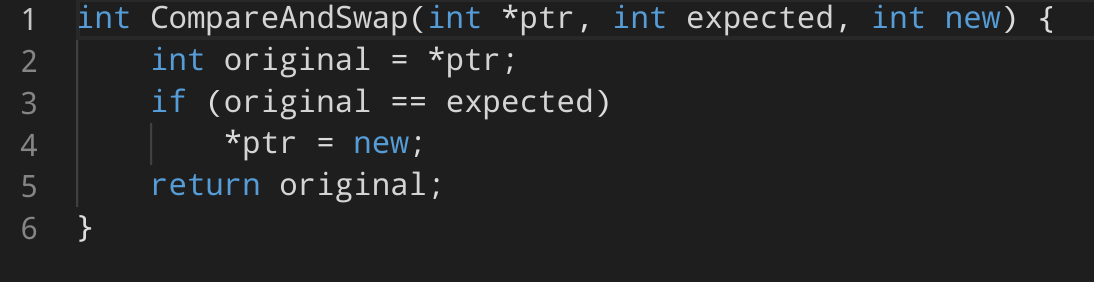
\includegraphics[width=0.65\textwidth]{chapters/Cucurrency/Cucurrency/compare_and_swap.png}

    With \tbi{Compare-And-Swap}, it is possible to build a spin clock

    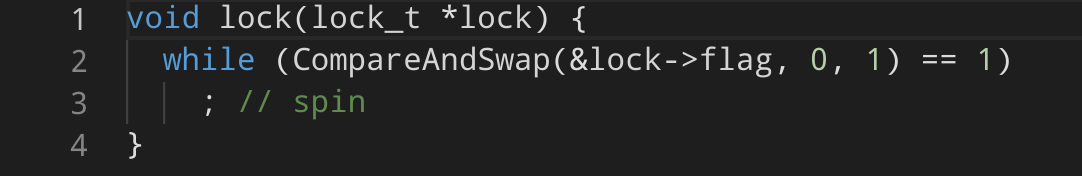
\includegraphics[width=0.65\textwidth]{chapters/Cucurrency/Cucurrency/compare_swap_spin_lock.png}

\sssc{Fetch-And-Add}

    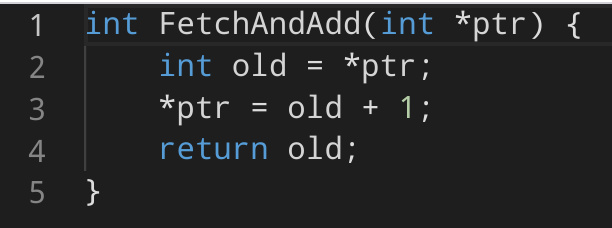
\includegraphics[width=0.6\textwidth]{chapters/Cucurrency/Cucurrency/fetch_and_add.png}

    And a spin clock can be build, a \tbi{ticket lock}

    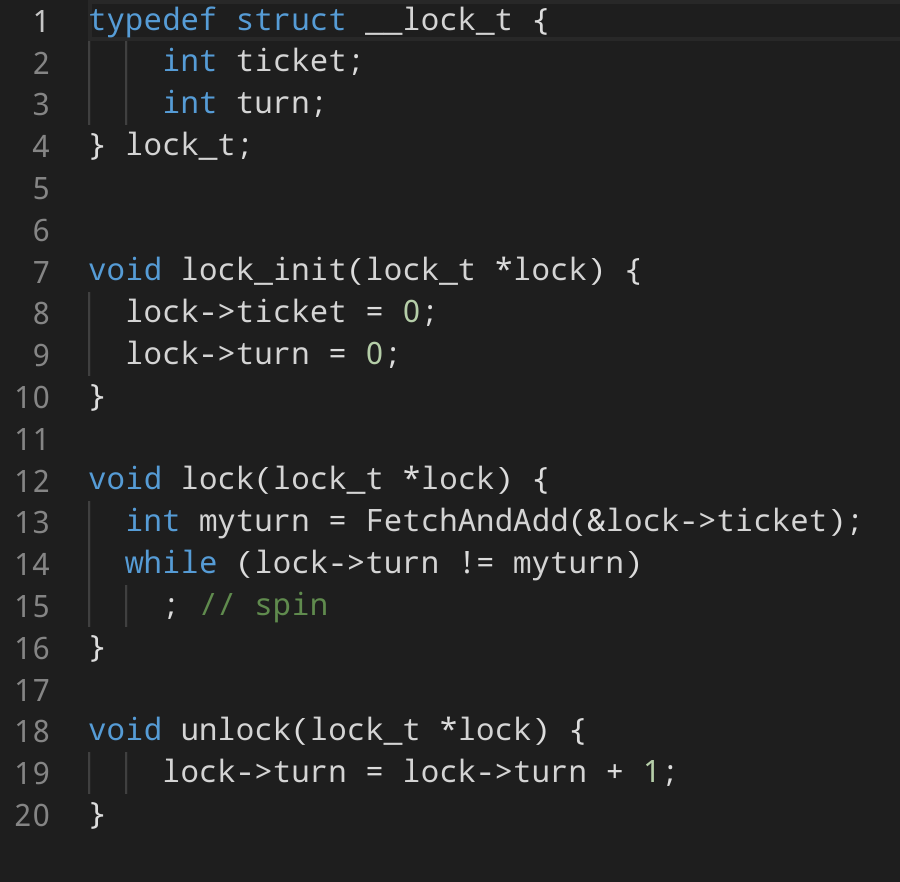
\includegraphics[width=0.6\textwidth]{chapters/Cucurrency/Cucurrency/ticket_lock.png}

    The advantage of \tbi{ticket lock} is that the approach "remeber" the requests of
    lock, i.e, it is like to pick a ticket that has number on it. And once the thread
    picks its ticket, all it needs to do is to wait and be called.

    $\Rightarrow$ this approach guarantees fairness.

    Other approaches are like fighting with each other for a single ticket.


\sssc{Spin locks and hardware limitation}

    With the extra hardware supports, we can now build spin locks. However the inefficiency is like 
    a diaster.

    Suppose each threads executes the same amount of time, with N threads and a single lock. The actual work
    done is $\frac{1}{N}$, and $\frac{N-1}{N}$ is useless busy-waiting.
    
    The hardware cannot solve everything, a smart software needs to be introduced in OS.

\sssc{Just yield, Baby}

    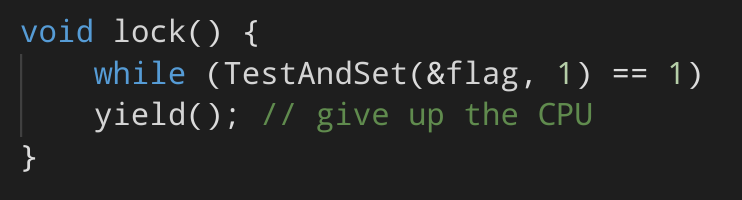
\includegraphics[width=0.5\textwidth]{chapters/Cucurrency/Cucurrency/yield.png}

    yield() is an operating system primitive which a thread can call when it wants to give up the CPU and 
    let another thread to run, i.e, descheduling the calling thread and move it from running to ready.

    
    \tbi{Efficiency Problem}:Suppose there are N threads and a single lock and the scheduler is taking round robin
    , N-1 yield would be called and only 1 critical section instruction would be executed. That is still 
    bad.

    \tbi{Fairness Problem}: If the scheduler is not using round robin, a thread would be picked consecutive to 
    call yield() which introduce the possibilty of starving a process.

\sssc{Using Queues: Sleeping Instead of Spinning}

    There are some controls needed over which thread next gets to acquire the lock after the current holder release
    it.

    Some OS support is need $\Rightarrow$ A queue to keep track of which threads are waiting to acquire the lock.

    \vspace*{2mm}
   
    \tbi{park()} and \tbi{unpark()}.

    In Solaris: \tbi{park()} to put a calling thread to sleep and \tbi{unpark(threadID)} to wake a particular
    thread as designated by \tbi{threadID}.

    When a thread tries to acquire the lock, the OS would park() to put the thread into sleeping and awakes it 
    by calling unpark(threadID) when the lock is free.

    
    \vspace*{2mm}
    
    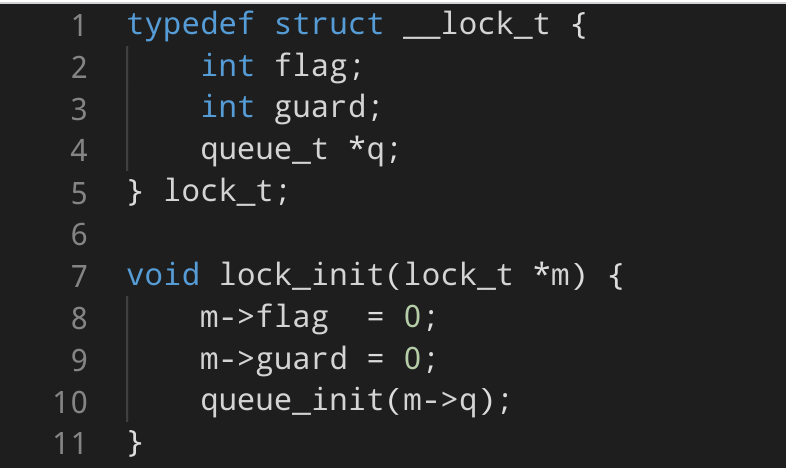
\includegraphics[width=0.6\textwidth]{chapters/Cucurrency/Cucurrency/lock_init.png}

    \tbi{Flag} indicates whether the lock is available, \tbi{guard} is used to ensure atomicity within 
    the lock()/unlock().

    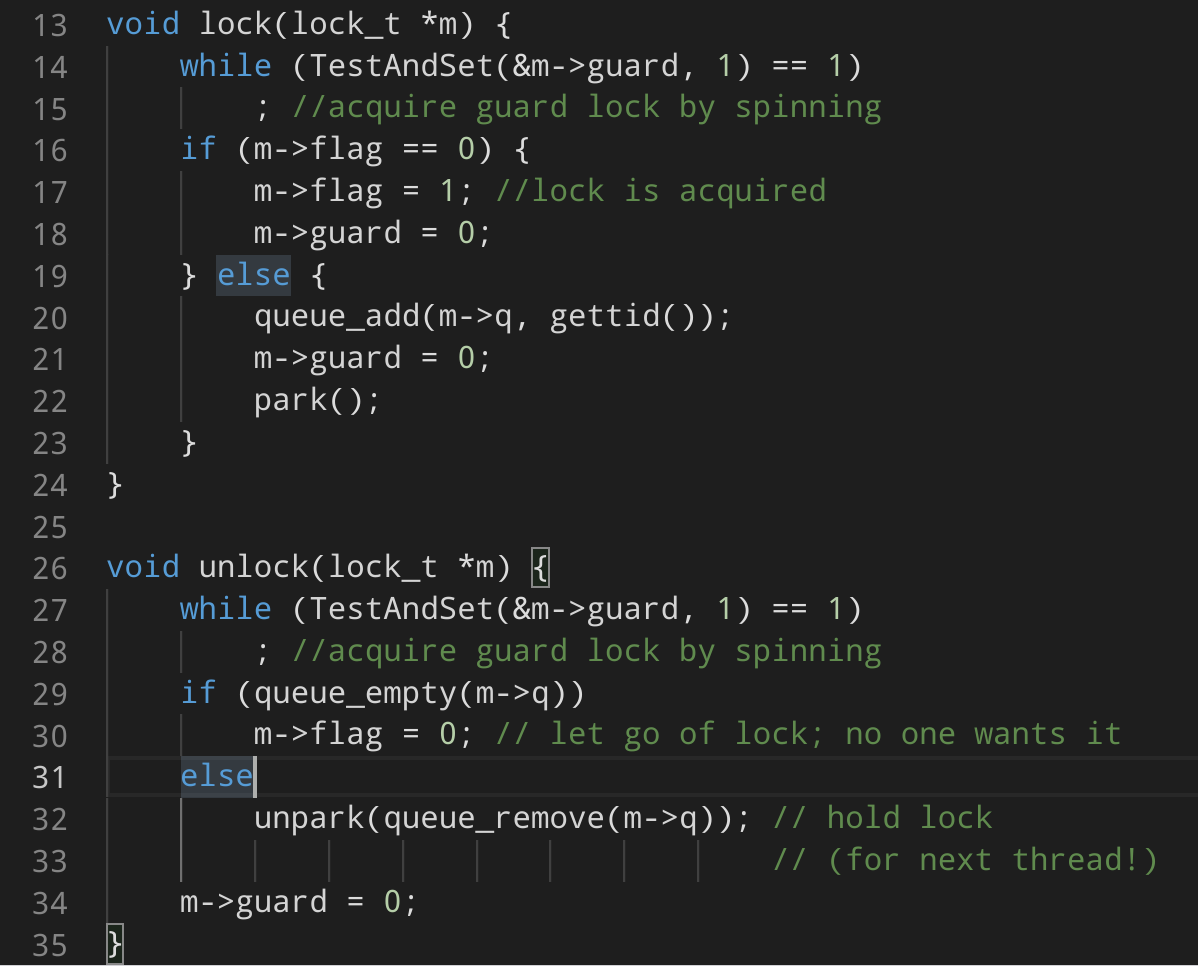
\includegraphics[width=0.7\textwidth]{chapters/Cucurrency/Cucurrency/park_unpark_approach.png}

    The guard is like another lock for the lock()/unlock(), one thread needs to hold the guard to acquire the 
    lock or put itself into sleep and release the guard.

    \vspace*{2mm}

    \tbi{Advantage:}
    \begin{enumerate}
        \item Small spinning/waste.
        \item Fairness by using the queue.
    \end{enumerate}

\sssc{Futex}

    A linux approach.... Kinda complicated, would take a look when studying linux.

    
\ssc{Locked Data Structures}

    We can use locks in some common data structures to make the structures thread safe.

\sssc{Cucurrent Counters}

    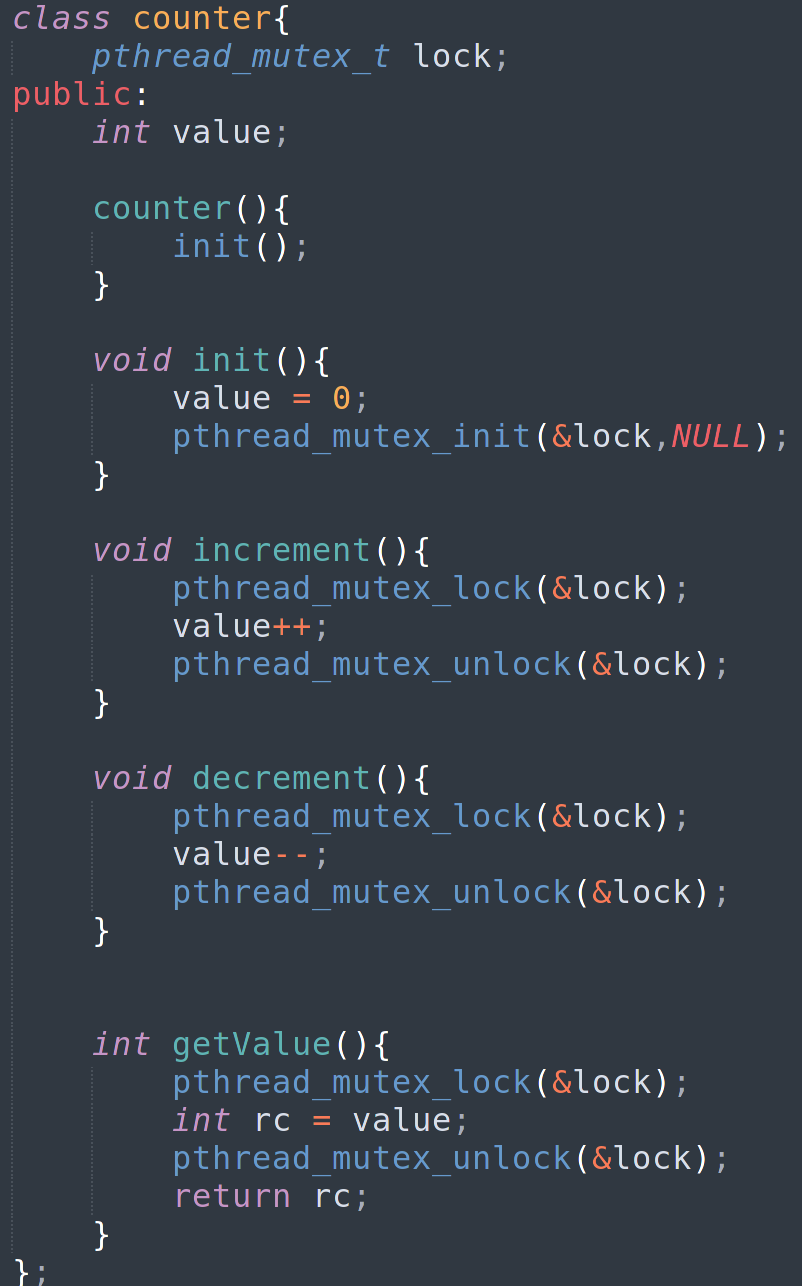
\includegraphics[width=0.5\textwidth]{chapters/Cucurrency/Cucurrency/current_counter.png}

    The lock is acquired and released automatically as you call and return from object methods, like
    a monitor.

    However, this approach scales poorly.

    \tbi{Approximate counters} works scablely. The idea is to give each thread a local counter, each thread 
    updates on its local counter, and when the counter reaches the threshold. It acquire the global lock 
    and accumulate its local counter to the global counter.

\sssc{Concurrent Linked Lists}

    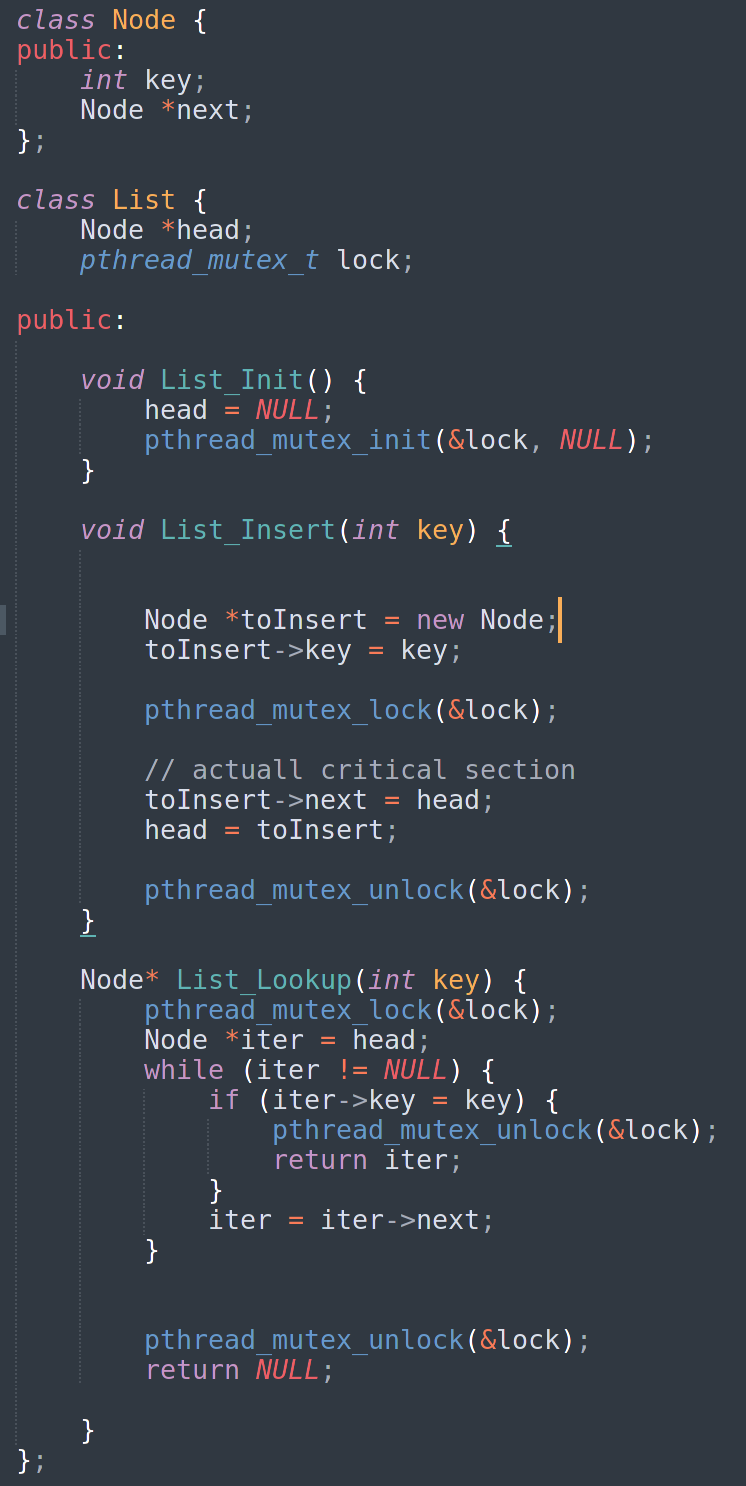
\includegraphics[width=0.5\textwidth]{chapters/Cucurrency/Cucurrency/cucurrent_linkedlist.png}

    However, this concurrent linked list is not scable.

    \tbi{Hand-over-hand locking} : Instead of having a single lock for the entire list, add a lock per node
    of the list. When traversing the list, the  code first grabs the next node's lock and then release the 
    current node's lock.(Potientially Deadlock).  Also, practically it is hard to make such a structure faster
    than the simple single lock approach, as the overheads of acquiring and releasing locks for each node is 
    prohibitive.

\sssc{Concurrent Queues}

    It is always standard to add a big lock to entire structure.

    Here is a more interesting concurrent queue designed by Michael and Scott: A lock for the head, and a lock for
    the tail.

    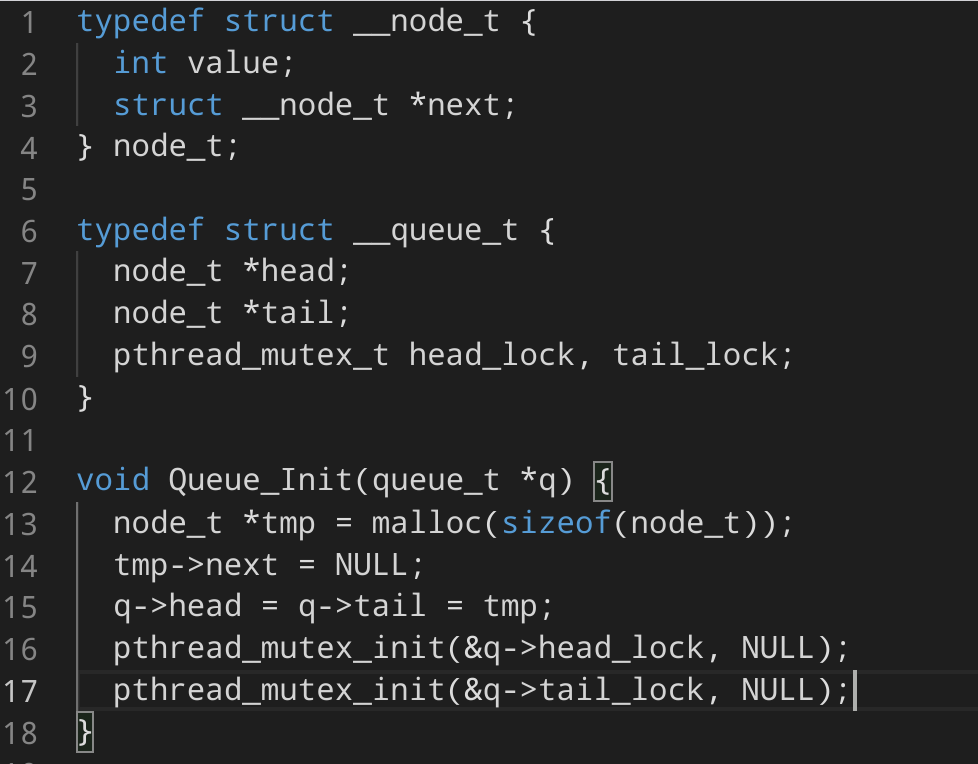
\includegraphics[width=0.5\textwidth]{chapters/Cucurrency/Cucurrency/concurrent_queue_init.png}
    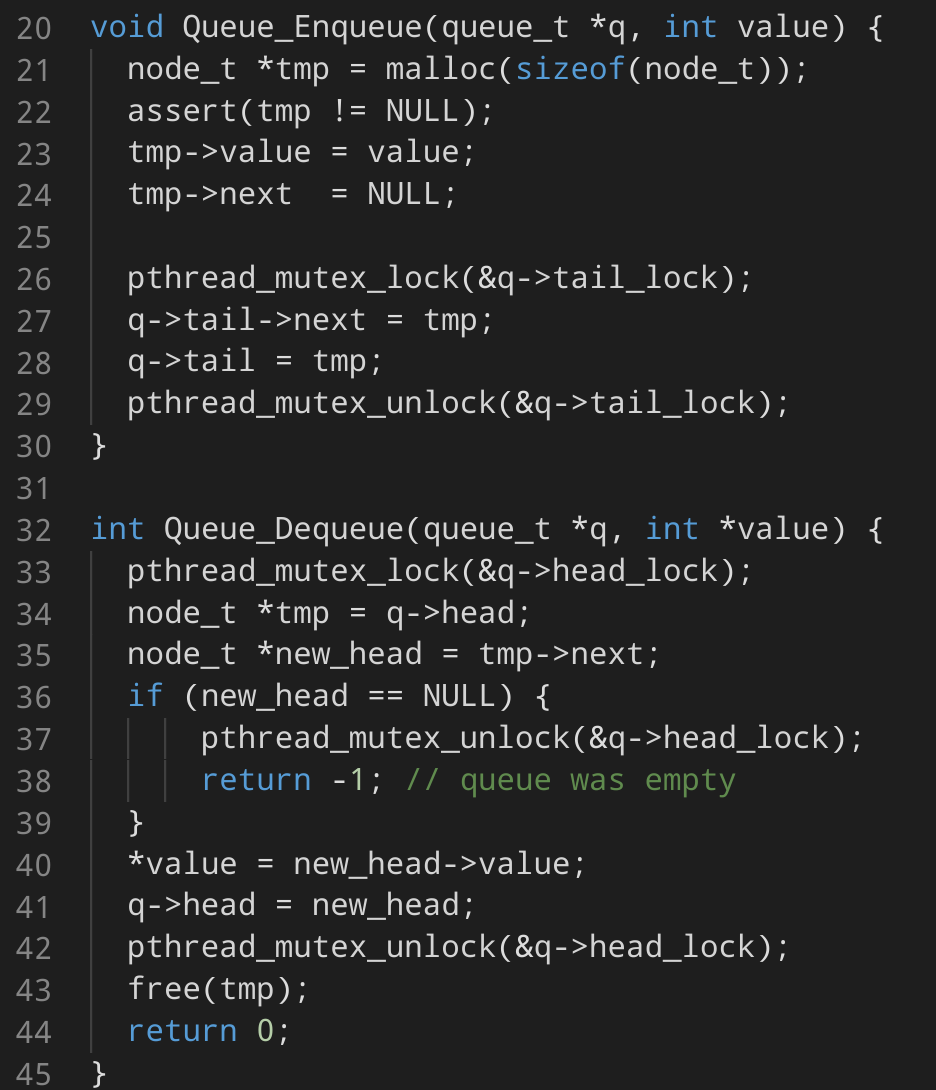
\includegraphics[width=0.5\textwidth]{chapters/Cucurrency/Cucurrency/concurrent_queue_operations.png}



\sssc{Concurrent Hash}

    A chaining hashtable is just an array of linked list. Since we have concurrent linked list,
    we could just use concurrent linked list to construct a hashtable. No more work needed.

    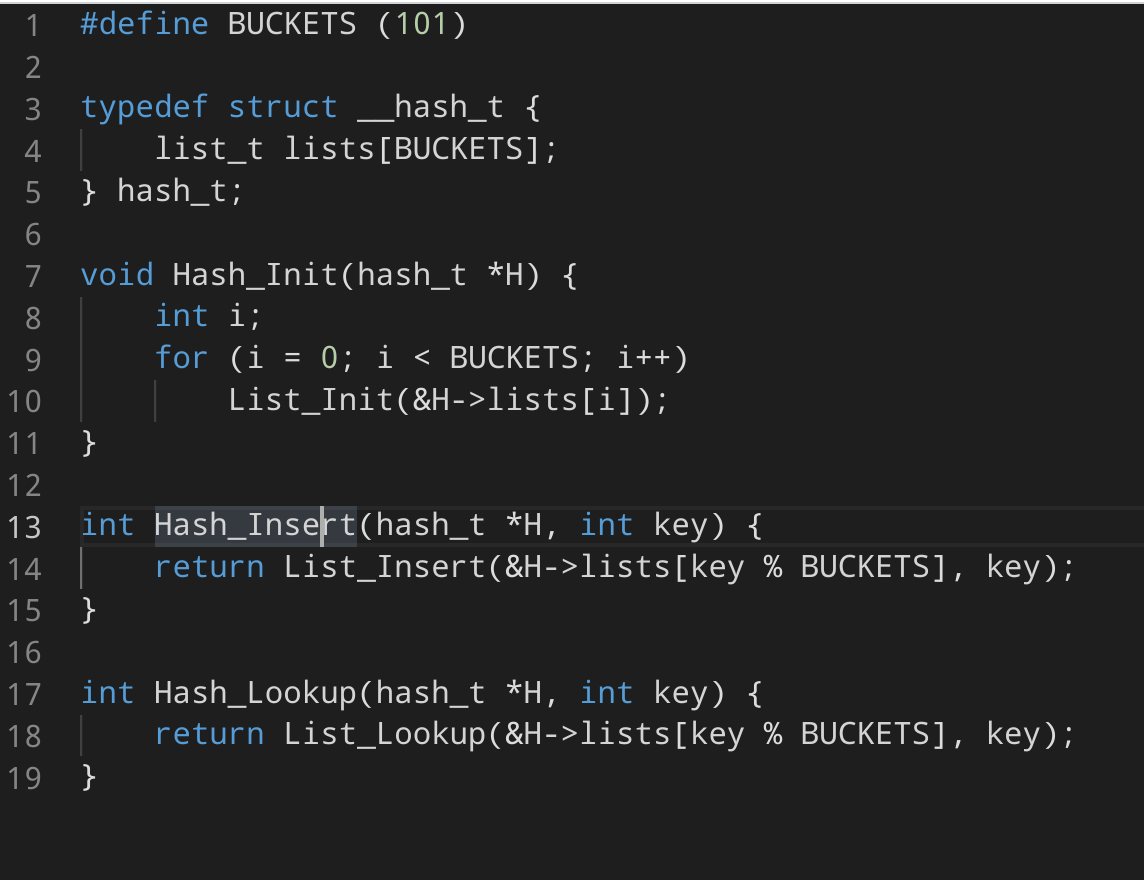
\includegraphics[width=0.5\textwidth]{chapters/Cucurrency/Cucurrency/concurrent_hashtable.png}


\ssc{Conditional Variables}

    There are many cases that we want to check whether a condition is true before continuing execute. 
    For exmaple, a parent thread would like to wait its children to finish execution using $pthread_join()$.

    A global conditional variable can used, and parent spins to wait the the global variable become true.
    However, we would like another approach that puts parent into sleep instead of spinning.

\sssc{Definition and Routines}

    A \tbi{condition variable} is an explict \tbi{queue} that threads can put themselves on 
    when some condition, which is not as desired by waiting on the condition.

    From my understanding, it a thread A is waiting for a state, it would put it into the queue that 
    every thread in the queues wants the same state. Thread B can make the state happen, and then thread 
    B would wake up one or more those threads in the queue, including A.

\sssc{Syntax and Usage}

    In pthread library, \tbi{$pthread cond_t$ name;} can be used to create condition variable. 
    
    And a condition variable has two operations: \tbi{wait()} and \tbi{signal}.

    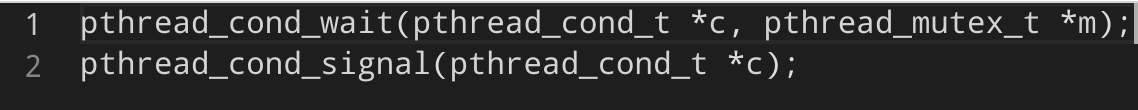
\includegraphics[width=0.4\textwidth]{chapters/Cucurrency/Cucurrency/wait_signal.png}

    \tbi{wait()} is like "Hey, I need something and put me into sleep until that thing is avaiable."

    \tbi{signal()} is like "Ok, I make the thing you wanted, and I am going to wake you up."

    Note that wait() takes a lock as second parameter, and that is because it assumes the lock 
    is hold by the caller when calling wait() and it would release the lock and be put into sleep
    (automically). The wait() won't return unless the lock is reacquired by the caller.

    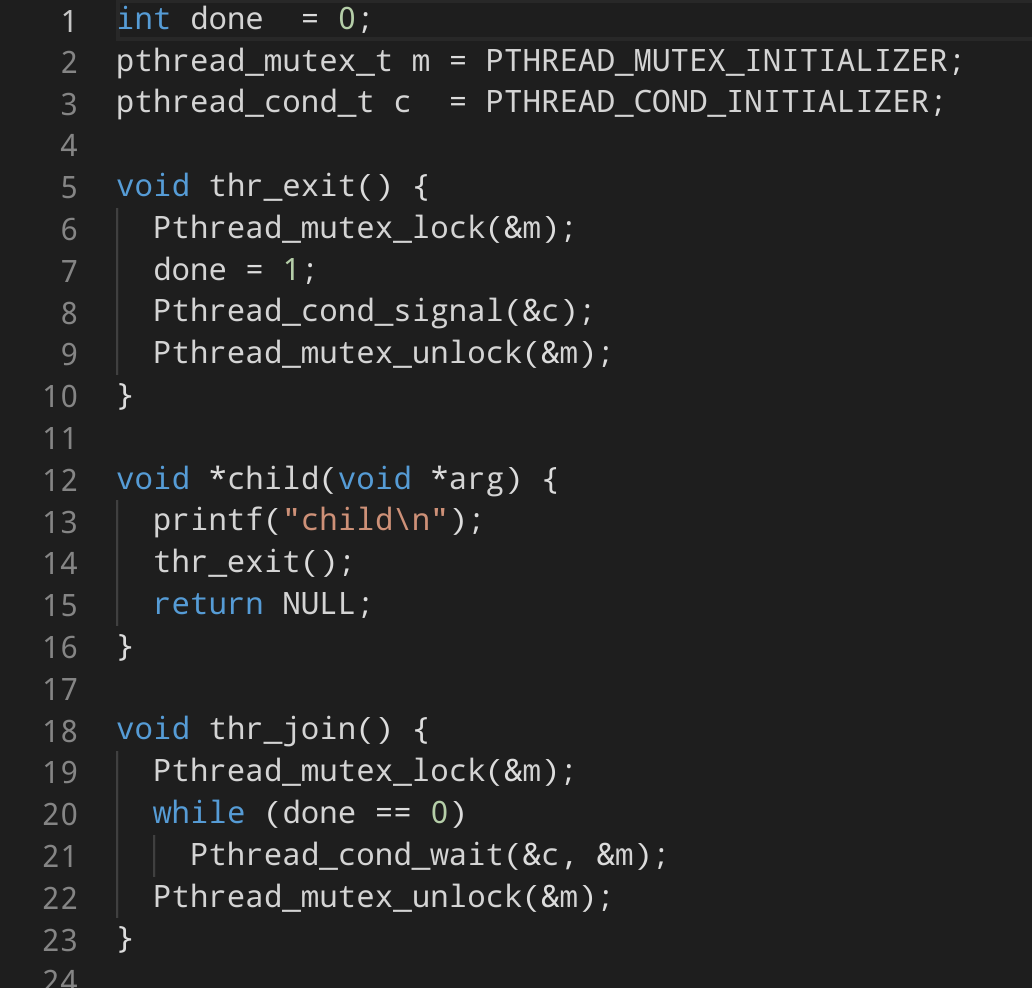
\includegraphics[width=0.65\textwidth]{chapters/Cucurrency/Cucurrency/thread_join_with_condition_variable.png}

    But, why! Why! Why we need the state variable?

    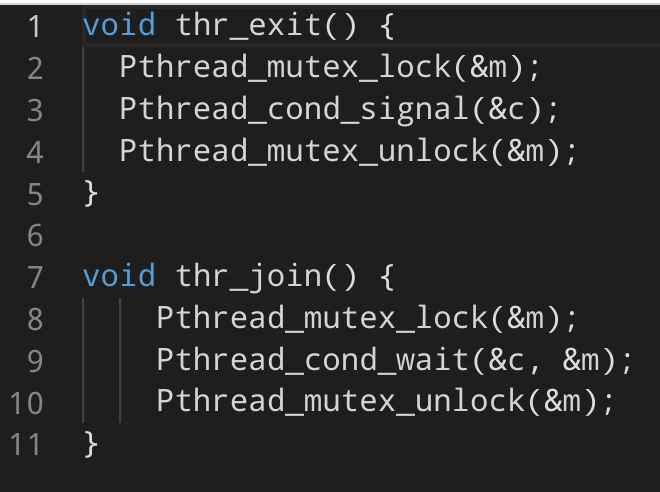
\includegraphics[width=0.6\textwidth]{chapters/Cucurrency/Cucurrency/importance_state_variable.png}

    Imagine, child thread executes upon the creation. It would signal when the queue is empty and exit.
    When the control is returned to the parent, parent would still call wait() and no one is going to 
    wake it up. A \tbi{If} instead a \tbi{While} would probabily makes much sense. 

    \tbi{TIP: Always Hold the Lock While Signaling}

    \tbi{Mandatory: Hold the Lock While Calling Wait}.

\sssc{Producer/Consumer (Bounded Buffer)}

    Problem Statement: Producers generate data items and place them in the buffer; consumers grab said items 
    from the buffer and consume them in some way.

    \underline{A real would example: Web server; A producer puts HTTP requests into a work queue. 
    While, the consumer threads
    take request out of the queue and process them.}


    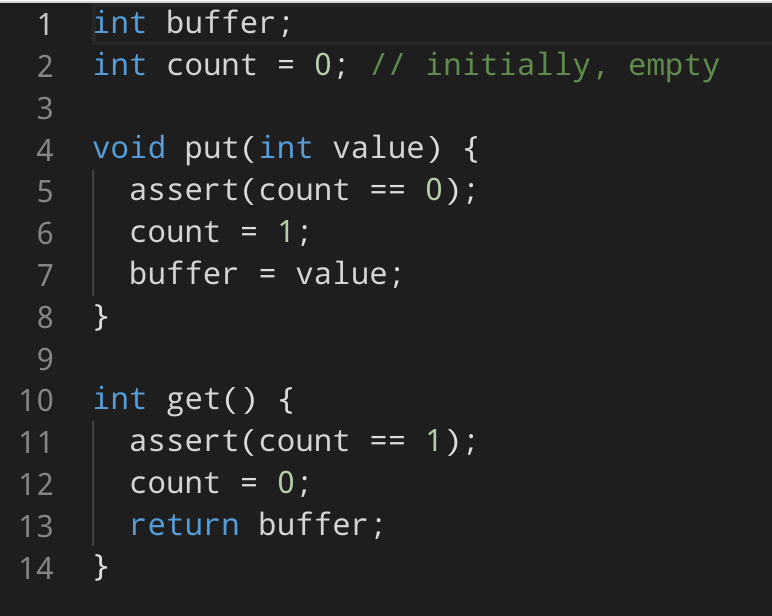
\includegraphics[width=0.55\textwidth]{chapters/Cucurrency/Cucurrency/put_and_get.png}
    
    We use int for simplicty. This buffer only has one slot for item. 
    put() should set count to 1 when the slot is empty and get() should set count to 0 when the slot is filled.

    \vspace*{5mm}

    \tbi{A broken approach:}

    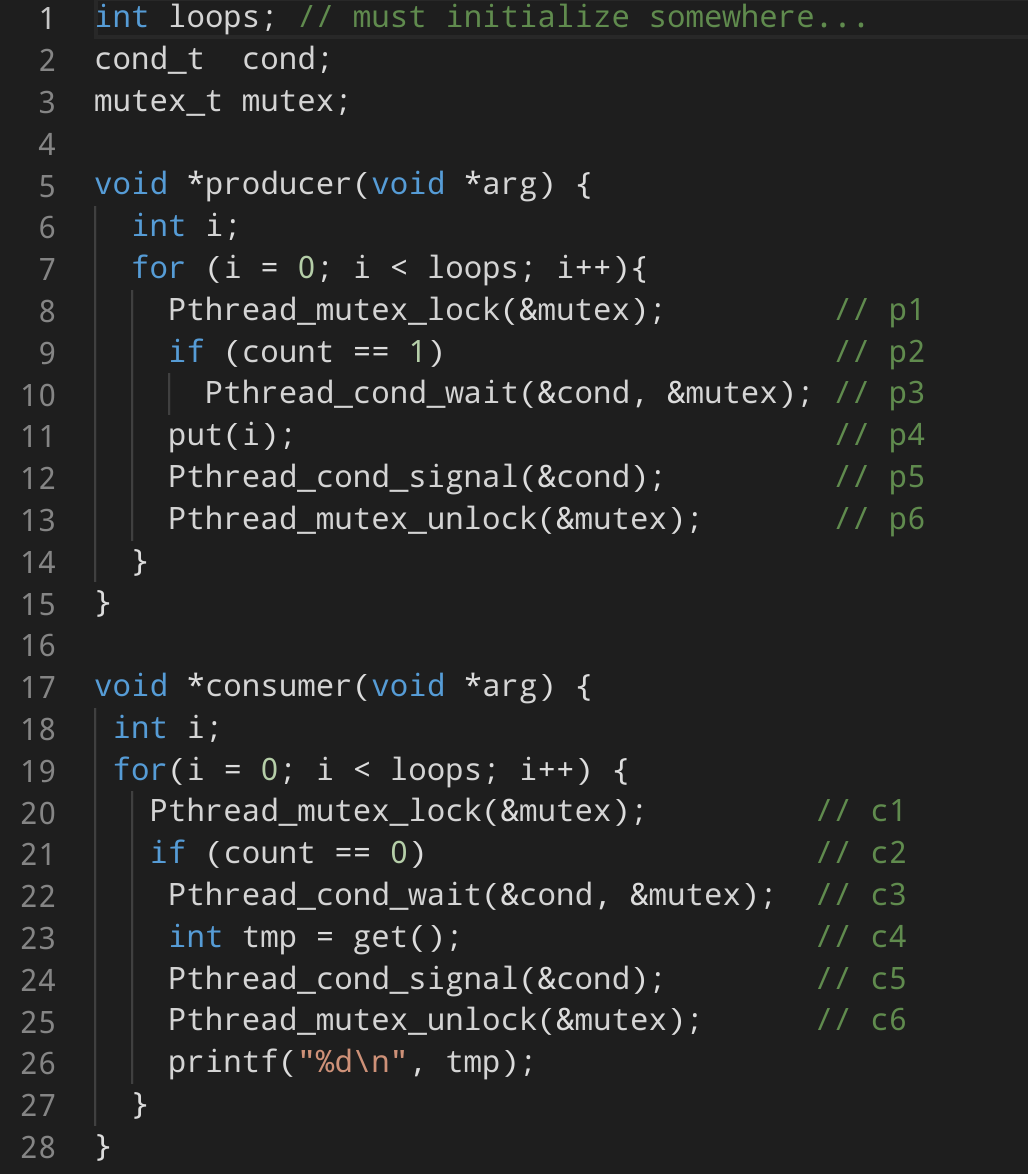
\includegraphics[width=0.65\textwidth]{chapters/Cucurrency/Cucurrency/pc_broken.png}

    This works only when there is exactly one producer and one consumer, since the condition variable is set 
    in a way that producer and consumer take turns.
    However, this is not useful anyway. Suppose there are two consumer c1,c2 and one producer p1.

    Upon the creation of the c1, it runs and check the buffer is empty it waits. Then p1 runs and put item 
    into the buffer and it call signal. Now c2 passed the if statement, and both c1,c2 call get().

    You see here, the signal only tells at the moment the world is desired and you can wake up. But when 
    waiting one wakes up, it could find the work has already changed once again, i.e, not desired.

    \vspace*{5mm}
    
    \tbi{A "better" broken approach: use while instead of if}

    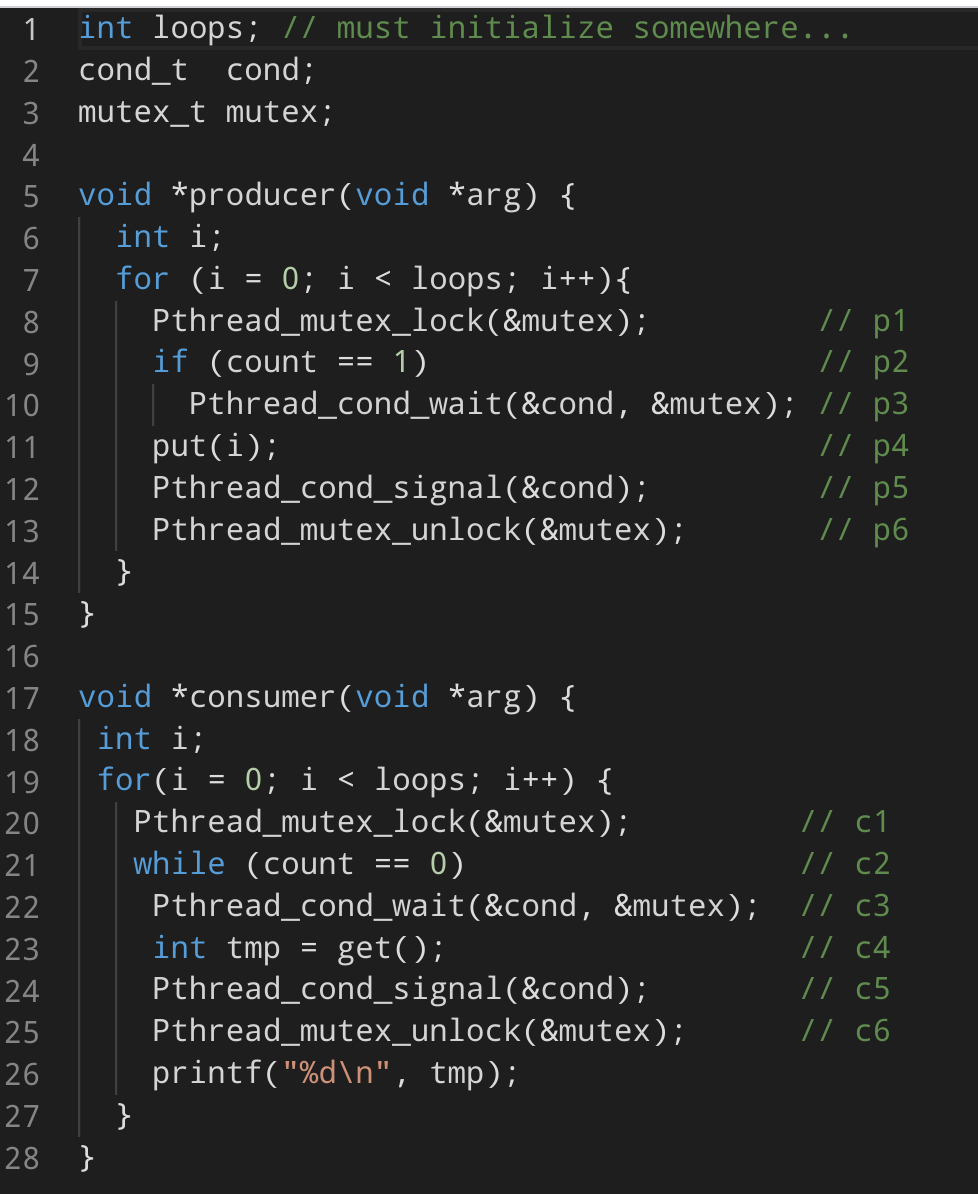
\includegraphics[width=0.65\textwidth]{chapters/Cucurrency/Cucurrency/better_broken_pc.png}

    This would address the issue in last approach, c1 and c2 can safely consume the product.
    When c1 wakes up, it checks whether the world is desired again (because of while). 

    This "always use while loops" is called \tbi{Mesa semantics}.

    However, the above approach is still broken due to the nondeterministic signaling.

    \begin{enumerate}
        \item both c1 and c2 sleep when they find there is item in the buffer.
        \item p1 puts the item in the buffer and signal one consumer to wake up, and go to sleep
        \item assume c1 wakes up, and cosumed the one item.
        \item c1 signals on the condition variable,and went to sleep.
        \item c2 wakes up, and check the buffer is empty, back to sleep.
        \item all p1,c1,c2 are sleeping
    \end{enumerate}

    This is due to there is one condition variable, and the signaling is nondeterministic. 
    A consumer should never wakes up a consumer, and a producer should never wake up a 
    producer.

    \vspace*{5mm}

    \tbi{Correct solution:}

    Producer wakes up consumer, and consumer wakes producer. Thus, two condition variables needed.

    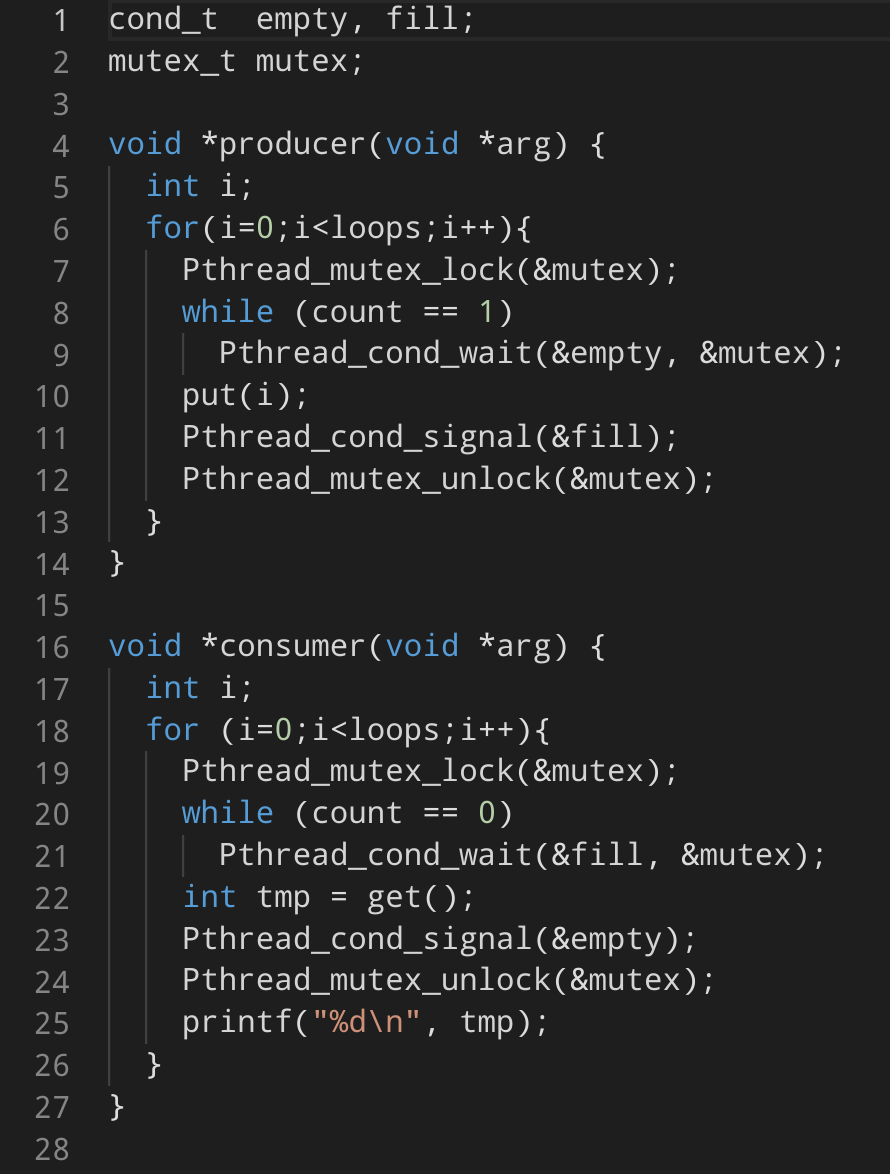
\includegraphics[width=0.6\textwidth]{chapters/Cucurrency/Cucurrency/two_condition_variable_solution.png}

    Note that two condition variables are in using: \tbi{empty} and \tbi{fill}, if is used to replace while in 
    producer part.

    When producer filled the buffer, it signals full "Hey, we have item in the buffer". And it waits for 
    empty "Well, call me when the buffer is empty".

    When consumer emptied the buffer, it signals empty "Hey, producer. The buffer is empty, please fill".
    And it waits for full "Also, call me when it is filled, I need more".

    \vspace*{5mm}

    \tbi{General solution:}

    We let producer produces multiple items when wakes up.
    And let consumer consumes multiple items when wakes up.

    With single pair of producer and consumer, this approach is more efficient as
    it reduces context switches; with multiple prodcuers or consumers, it even allows
    concurrent producing or consuming to take place.

    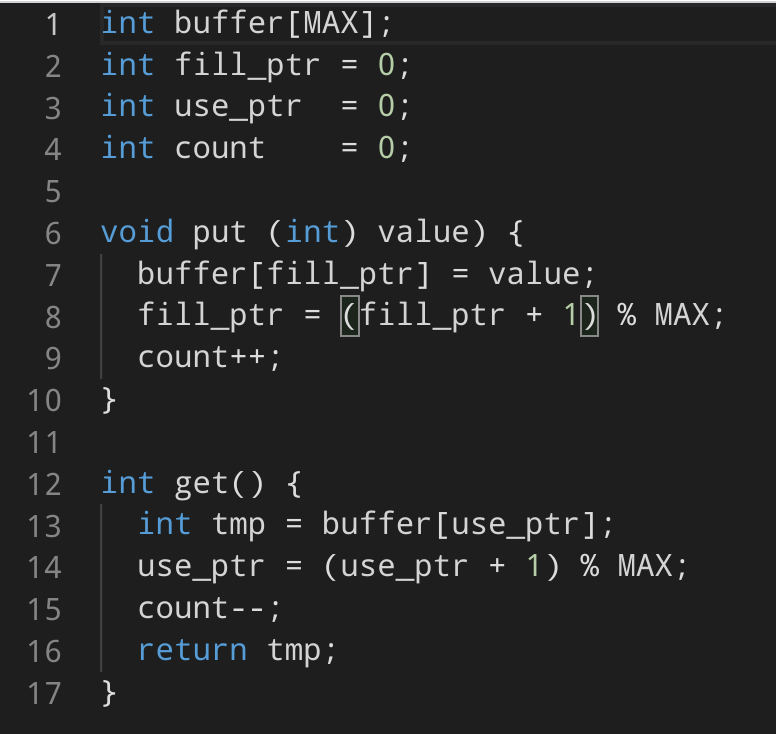
\includegraphics[width=0.45\textwidth]{chapters/Cucurrency/Cucurrency/revised_get_and_put.png}
    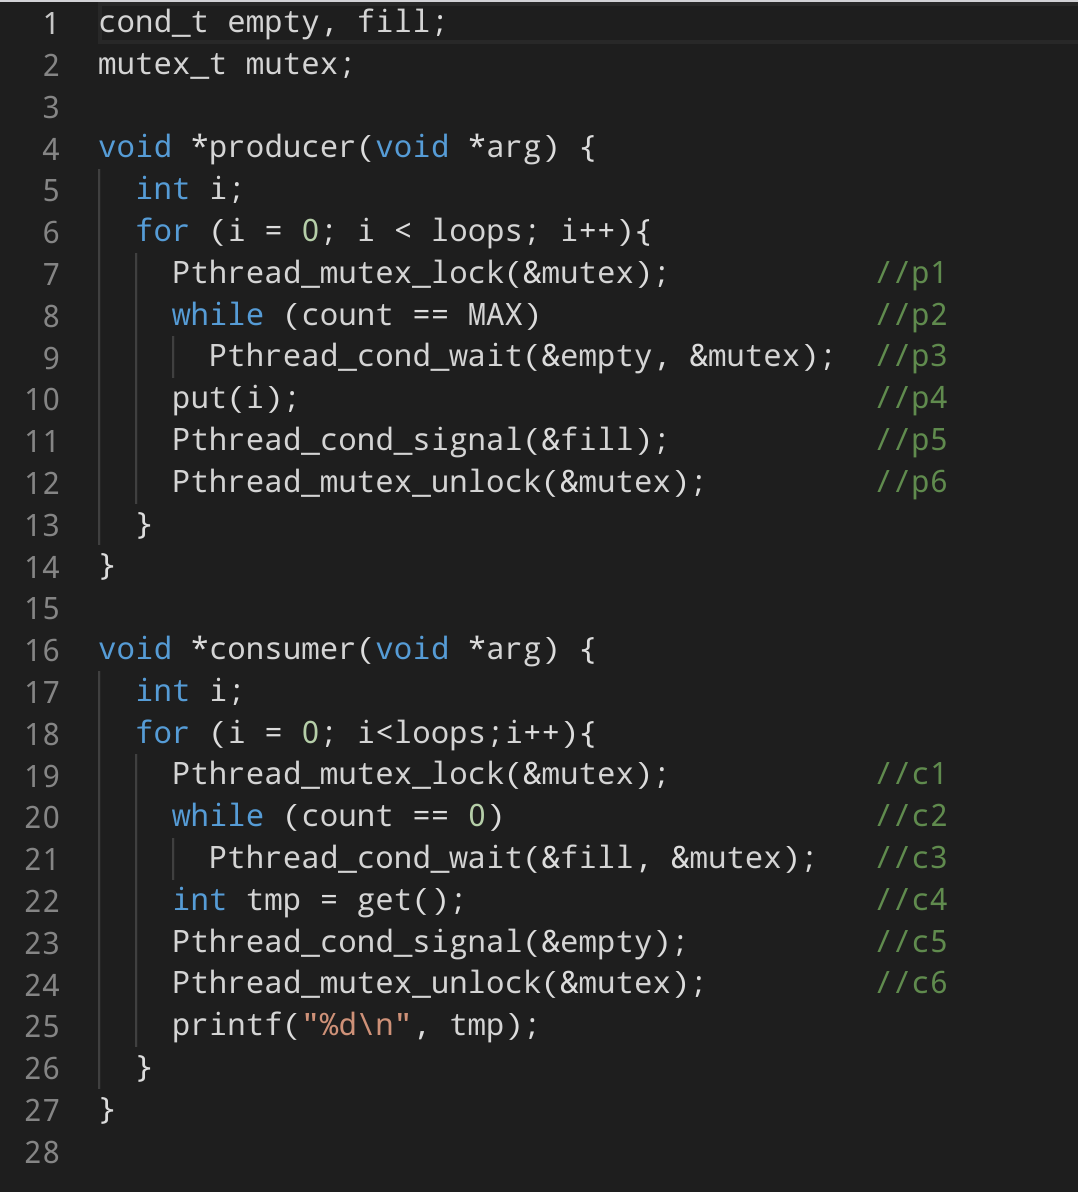
\includegraphics[width=0.50\textwidth]{chapters/Cucurrency/Cucurrency/revised_producer_consumer.png}

\sssc{Covering Conditions: Broadcast}

    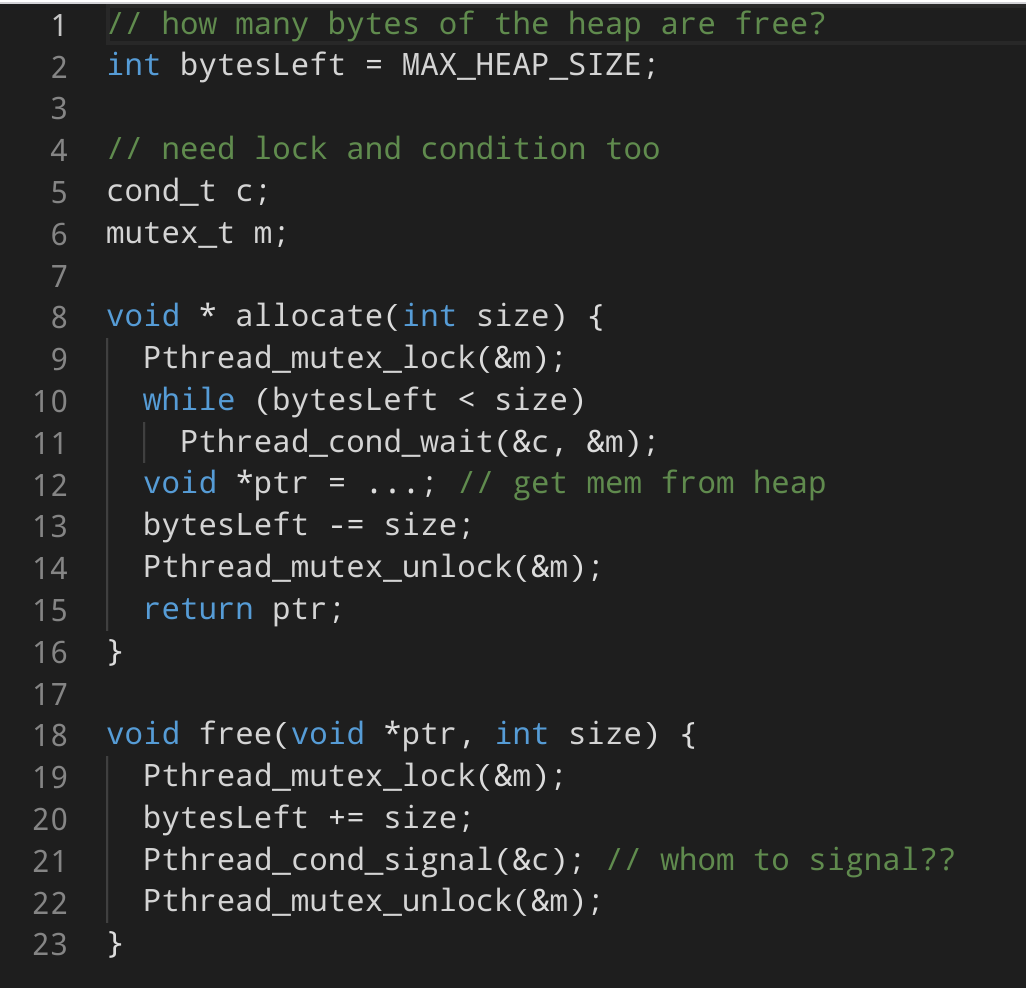
\includegraphics[width=0.55\textwidth]{chapters/Cucurrency/Cucurrency/covering_conditions.png}

    Problem Scenario:

    There are two threads Ta,Tb. Ta asks for 10 bytes and Tb asks for 100 bytes. At the creations of Ta and 
    Tb, there is 0 bytes free memory. Therefore Ta and Tb sleep. When Tf frees up 50 bytes, Tf signaled 
    Tb which needs 100 bytes. Tb would sleep again, and no memory would be allocated even Ta's request 
    can be fulfilled.\\

    Solution: 

    Instead of \textbf{$pthread_cond_signal()$}, we can use \textbf{$pthread_cond_broadcast$}.

    However, the cost is very noticable since all threads would be waken up.


\ssc{Semaphore}

\sssc{Definition:}
    
    A semaphore is an object with an integer value that we can manipulate with 
    two routines; in POSIX, these routines are \tbi{$sem_wait()$} and
     \tbi{$sem_post$}.

    The initial value of the semaphore determines its behavior, it is necessary
    to initialize the semaphore to some value.

    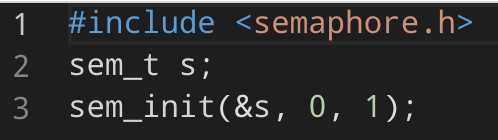
\includegraphics[width=0.55\textwidth]{chapters/Cucurrency/Cucurrency/semaphore_init.png}

    After initialize the semaphore, one can interact with it using \tbi{$sem_wait()$} and
    \tbi{$sem_post$}.

    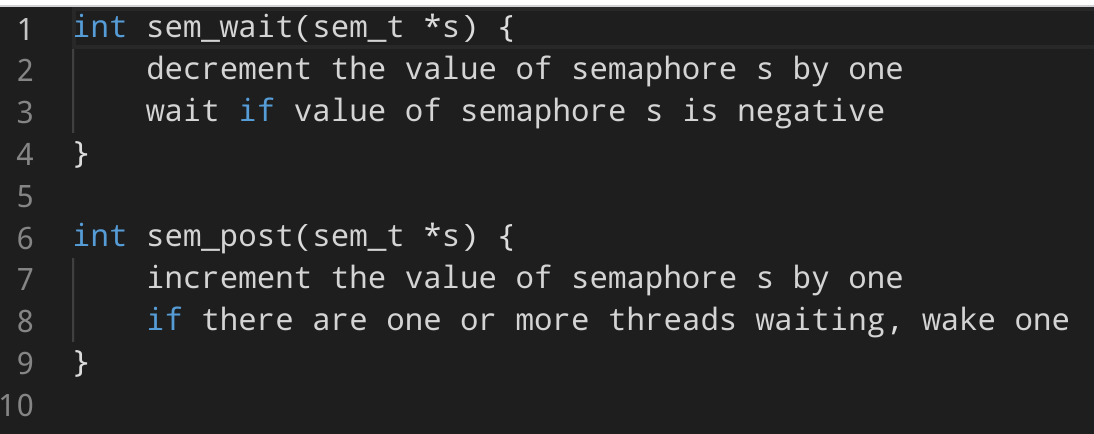
\includegraphics[width=0.60\textwidth]{chapters/Cucurrency/Cucurrency/semaphore_routines.png}

    \underline{\textbf{The value of the semaphore is equal to the number of,
    when negative,waiting threads.}}

    And the initial value is the number of resources that can be give away at start.
\sssc{Binary Semaphore (Locks)}

    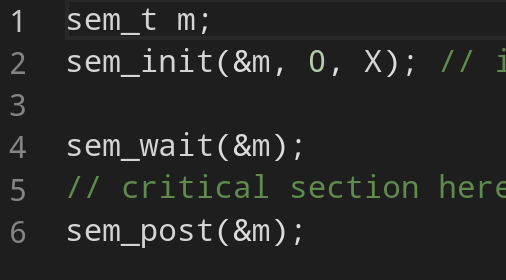
\includegraphics[width=0.6\textwidth]{chapters/Cucurrency/Cucurrency/binary_semaphore.png}

    This is essential just a lock, when semaphore is initialized to 1.

    However, this is useless since the lock already serves the purpose.

\sssc{Producer/Consumer (Bound Buffer):Semaphore approach}

    Note that semaphore works like a combination of lock and condition variable.

    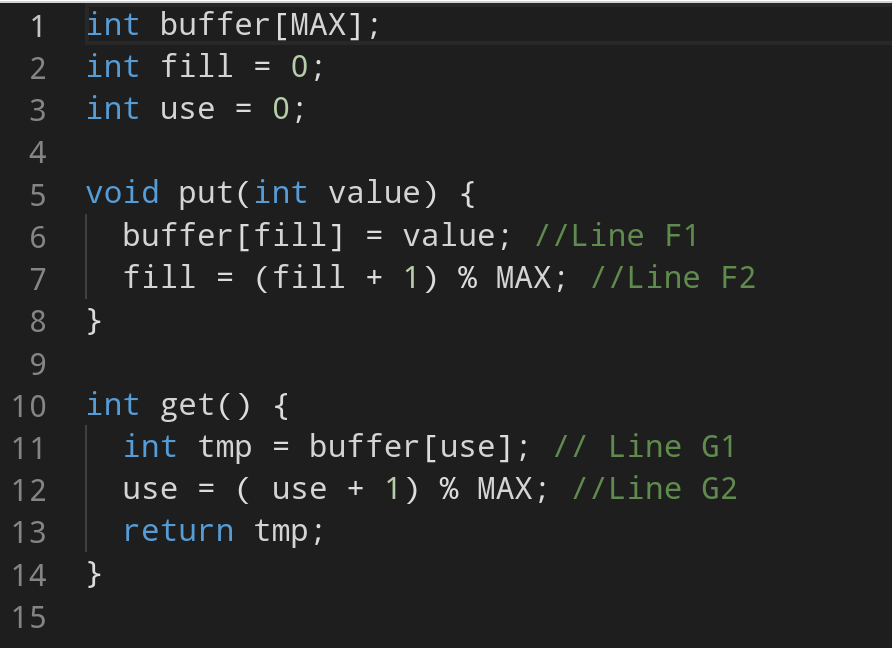
\includegraphics[width=0.5\textwidth]{chapters/Cucurrency/Cucurrency/pc_semaphore_get_put.png}

    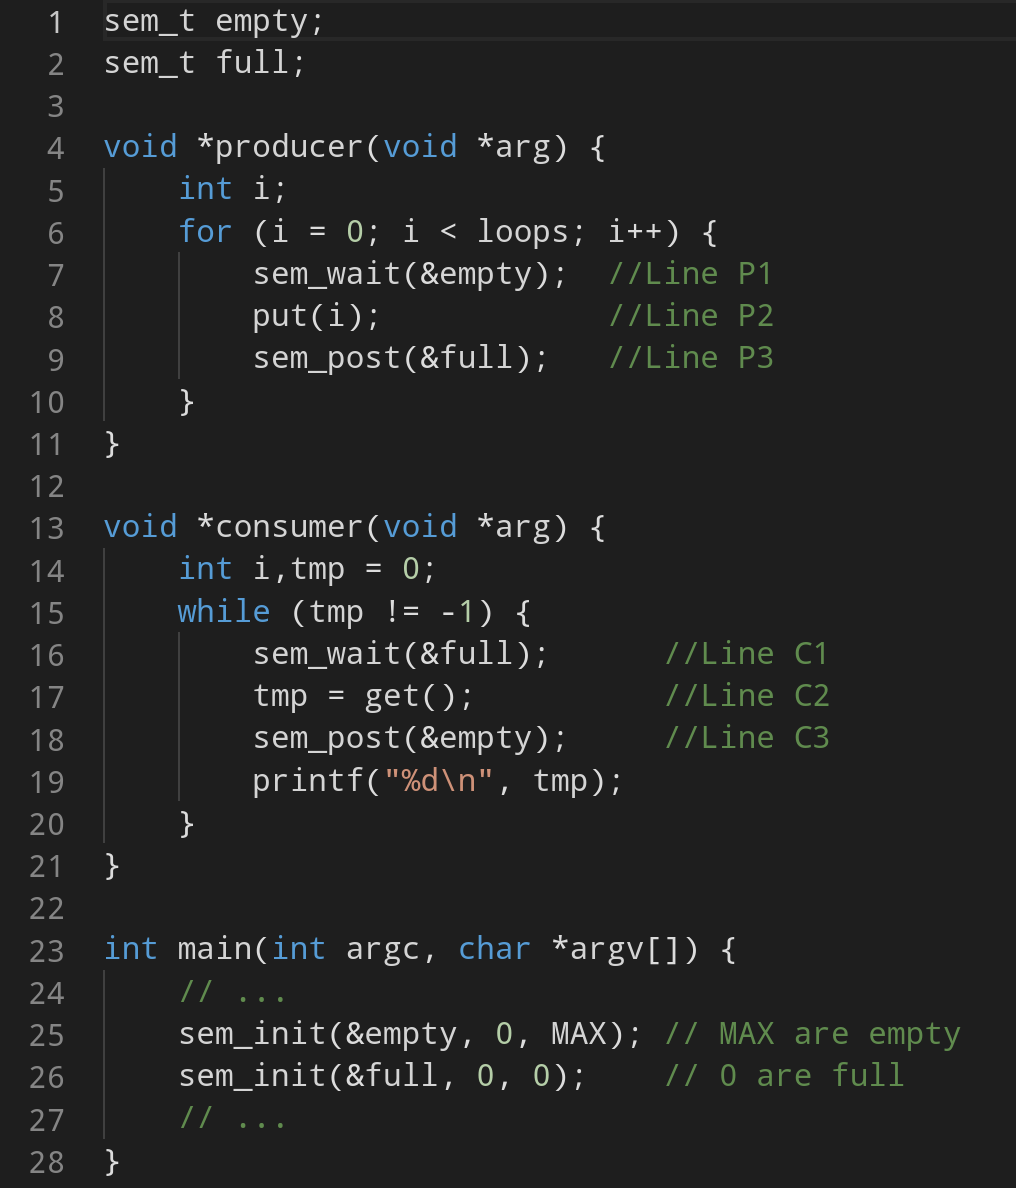
\includegraphics[width=0.5\textwidth]{chapters/Cucurrency/Cucurrency/pc_semaphore.png}

    However, there would be a race condition at the put() and get():
    \begin{enumerate}
        \item Pa gets to run get() first, it first puts item in slot i.
        \item just before Pa increment the slot counter, it gets interrupted.
        \item Pb still have slot counter at slot i, and Pb overwrites slot i.
    \end{enumerate}

    That is , there is no mutual exclusion for put() and get(), but only signaling
    whether one can put or get.

    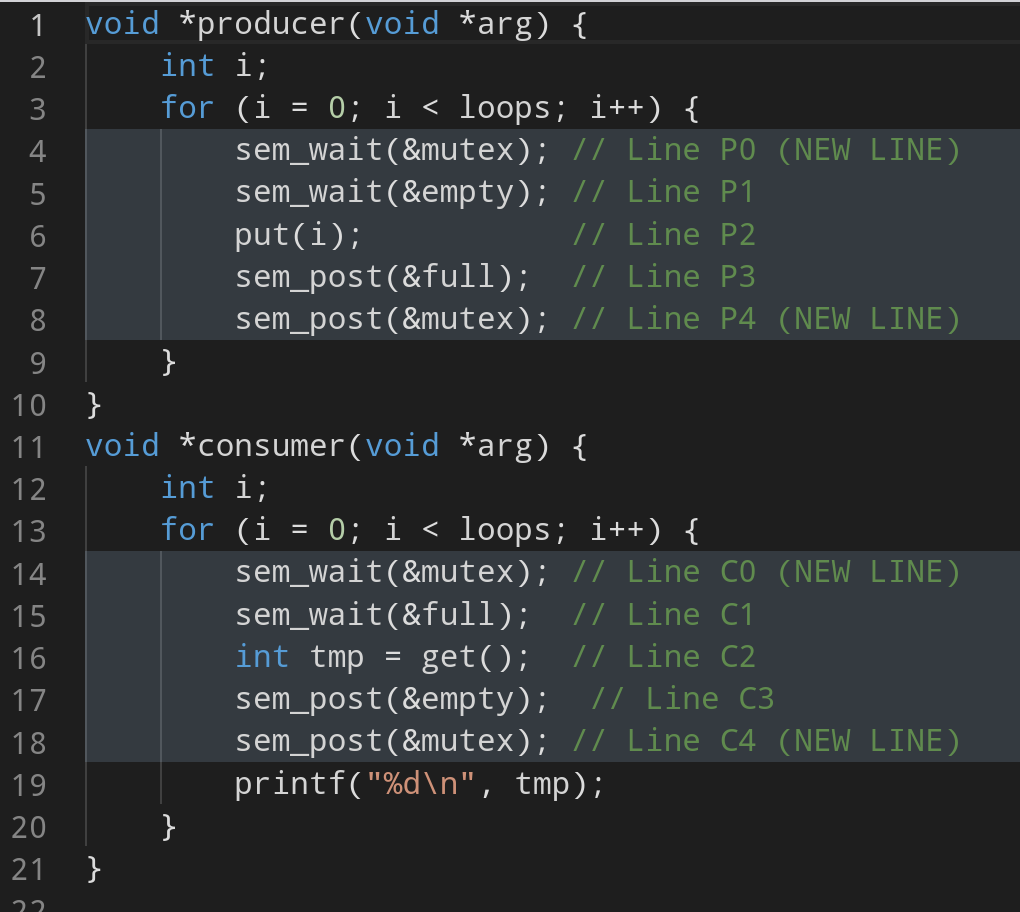
\includegraphics[width=0.6\textwidth]{chapters/Cucurrency/Cucurrency/revised_pc_semaphore.png}

    Now, the revised solution use semaphore (like a lock) to add mutual exclusion.

    \underline{\textbf{However, it still doesn't work because deadlock since semaphore don't increament itself when sleep}} The consumers 
    and producers share a single lock.

    \begin{enumerate}
        \item Consumer C1 runs first, the use sem-wait(\&mutex) to required the lock, mutex = 0.
        \item C1 continue, and calls sem-wait(\&full), however there is no item in the 
        slot. And C1 sleeps.
        \item When any other producers or consumers try to do something, they don't have the lock,
        any sem-wait(\$mutex) would decrease the mutex to negative value and sleeps forever.
    \end{enumerate}

    Now a truly working vision,
    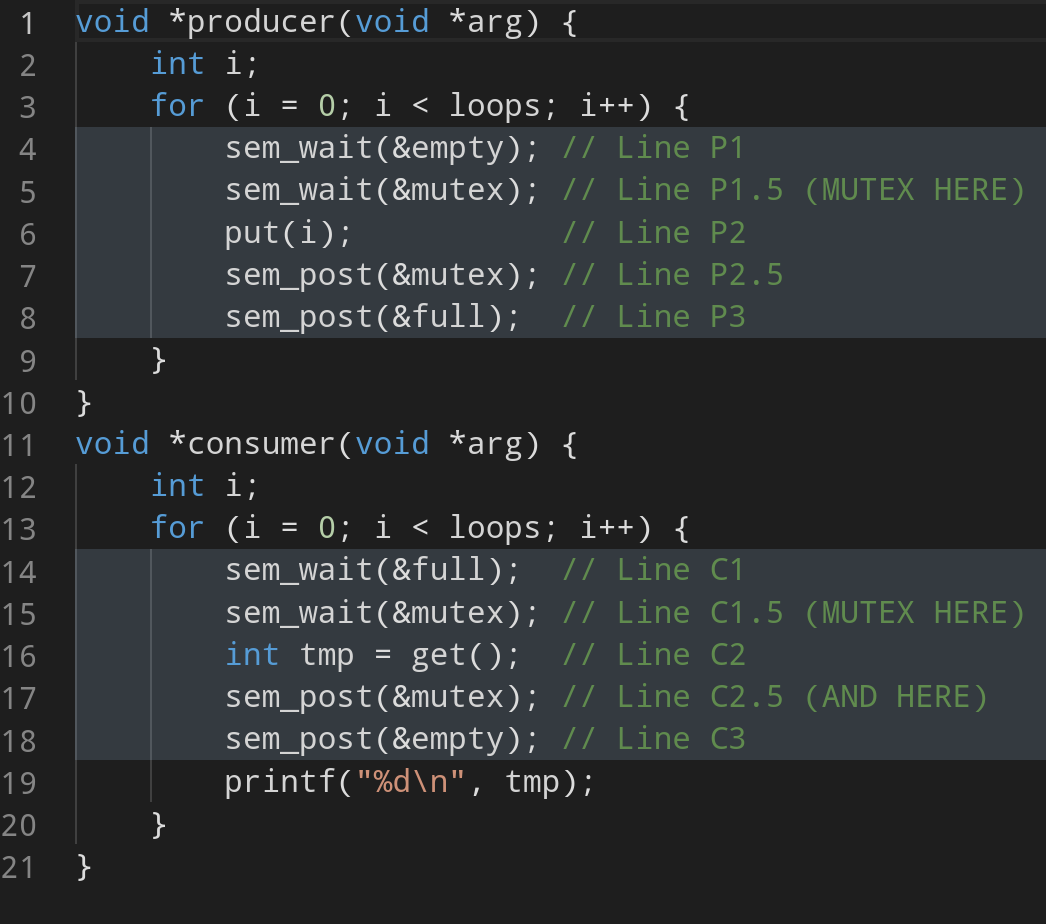
\includegraphics[width=0.5\textwidth]{chapters/Cucurrency/Cucurrency/true_revised_pc_semaphore.png}

    \underline{\textbf{To resolve the deadlock, simply reduce the scope of lock at this case}}.


\sssc{Reader-Writer Locks}

    For concurrent list operations, we need to guarantee that no two insertion races,
    but it is ok for multiple readers to lookup concurrently.

    \textbf{reader-write lock}: The implementation is in reader-writer.cpp

\sssc{Dining Philosophers}

    Problem statement: 
    There are five “philosophers” sitting around a table. 
    Between each pair of philosophers is a single fork (and thus, five total). 
    The philosophers each have times where they think and don’t need any forks, 
    and times where they eat. In order to eat, a philosopher needs two forks, 
    both the one on their left and the one on their right

    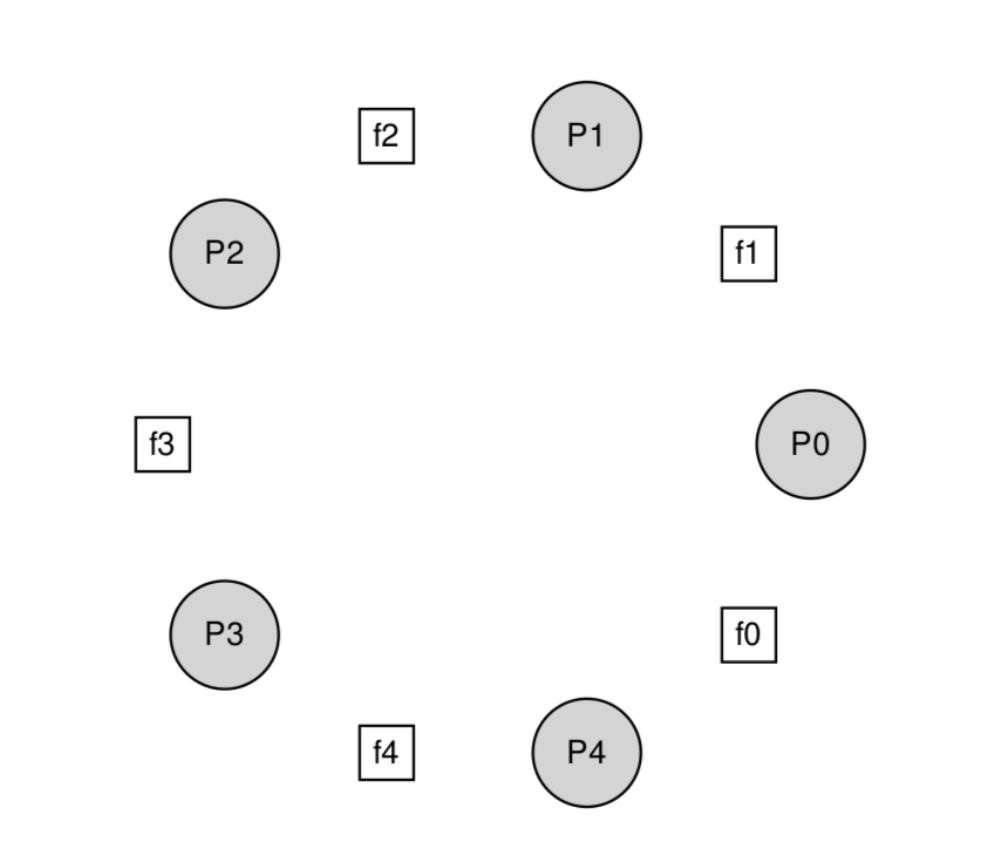
\includegraphics[width=0.5\textwidth]{chapters/Cucurrency/Cucurrency/dining_philosophers.png}

    Here is the behavior for a philosopher:

    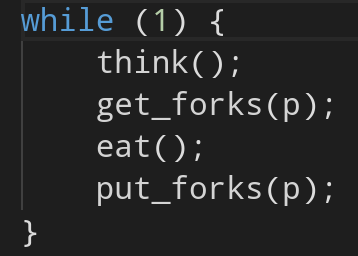
\includegraphics[width=0.5\textwidth]{chapters/Cucurrency/Cucurrency/dp_indiv.png}

    Some help functions needed

    \begin{lstlisting}
        int left(int p){
            return p;
        }

        int right(int p){
            return (p+1)%5;
        }
    \end{lstlisting}

    \textbf{Broken solution:}

    \begin{lstlisting}
        // potientially deadlock: if every philosopher grabs the left one
        // that is, all threads makes to sem_wait(&forks[left(p)]) and no further
        void get_forks(int p){
            sem_wait(&forks[left(p)]);
            sem_wait(&forks[right(p)]);
        }

        void put_forks(int p){
            sem_post(&forks[left(p)]);
            sem_post(&forks[right(p)]);
        }
    \end{lstlisting}

    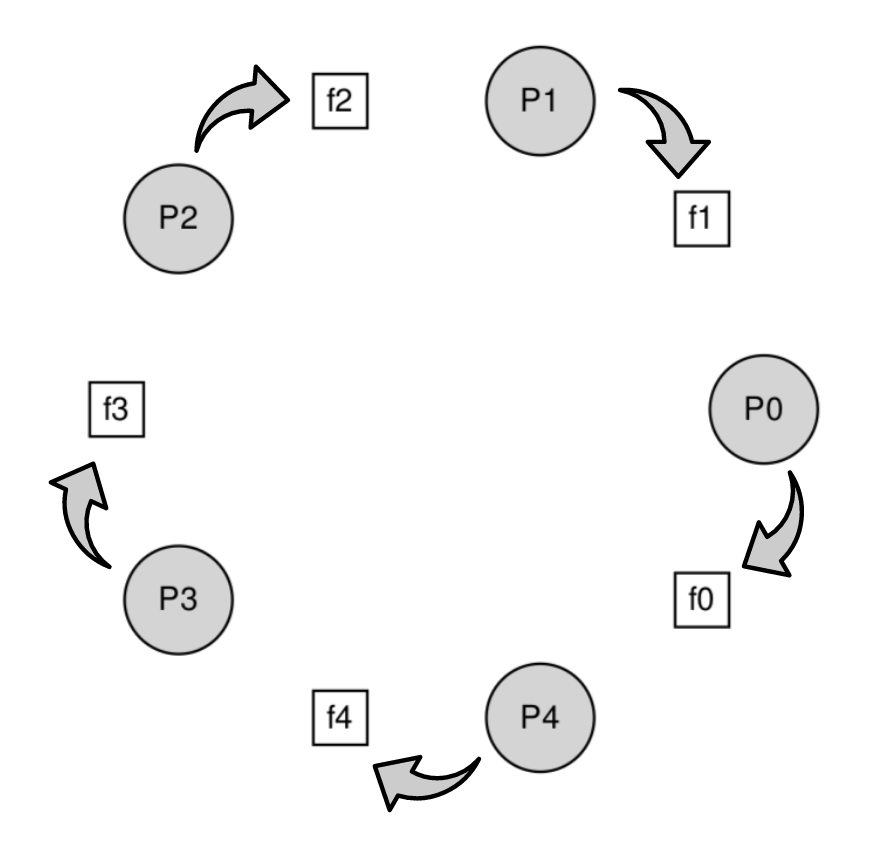
\includegraphics[width=0.5\textwidth]{chapters/Cucurrency/Cucurrency/dp_deadlock.png}

    \textbf{Dijkstra solution: break the dependency}

    Make one philosopher behaves different than other ones.

    \begin{lstlisting}
        void get_forks(int p){
            // letting philosopher 4 behaves differently, there would be deadlock
            // since there won't be a circle now.
            if(p==4){
                sem_wait(&forks[right(p)]);
                sem_wait(&forks[left(p)]);
            }else{
                sem_wait(&forks[left(p)]);
                sem_wait(&forks[right(p)]);
            }
        }
    \end{lstlisting}

\sssc{Thread Throttling}

    How can a programmer prevent "too many" threads from doing something at once and 
    bogging the system down?

    Answer is \textbf{Throttling:} decide a threshold, use semaphore to limit the number of threads 
    concurrently executing.

\sssc{How implement semaphore}

    \begin{lstlisting}
        typedef struct Semaphore{
            int value;
            pthread_cond_t cond;
            pthread_mutex_t lock;
        }semaphore;

        void sem_init(sem *s, int value){
            s-> value = value;
            cond_init(&s->cond);
            mutex_init(&s->lock);
        }

        void sem_wait(sem *s){
            pthread_mutex_lock(&s->lock);

            // however, this value would never go negative
            // easy to implement, linux's approach
            while(s->value <=0){
                pthread_cond_wait(&s->cond,&s->lock);
            }
            s->value = s->value - 1;
            pthread_mutex_unlock(&s->lock);
        }

        void sem_post(sem *s){
            pthread_mutex_lock(&s->lock);
            s->value = s->value - 1;
            pthread_cond_signal(&s-cond);
            pthread_mutex_unlock(&s->lock);
        }

    \end{lstlisting}


\ssc{Deadlock bugs}

    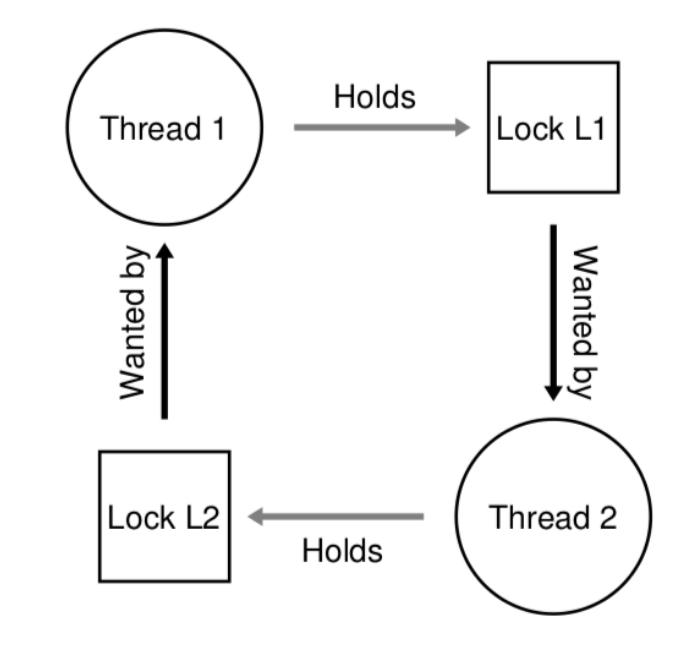
\includegraphics[width=0.5\textwidth]{chapters/Cucurrency/Cucurrency/simple_deadlock.png}

    \textbf{Four condtions} need to be hold for a deadlock to occur:

    \begin{enumerate}
        \item \textbf{Mutual exclusion:} Threads claim exclusive control of resources.
        \item \textbf{Hold-and-wait:} Threads hold the resource and wait for other necessary resource, wont let go.
        \item \textbf{No preemption:} Resources cannot be forcibly removed from the threads that are holding them.
        \item \textbf{Circular wait:} There exists a circular chain of threads such that each threads holds one or more 
        resources that are being requested by the next thread in the chain.
    \end{enumerate}

\sssc{Prevention}

    Make one of the four condition false all the time to prevent deadlock. However,
    this is not practical. 

\sssc{Deadlock avoidance via Scheduling}

    Instead of deadlock prevention, in some scenarios deadlock avoidance is preferable.
    Avoidance requires some global knowledge of which locks various 
    threads might grab during their execution, and subsequently,
    schedules said threads in a way as to guarantee no deadlock can occur.


    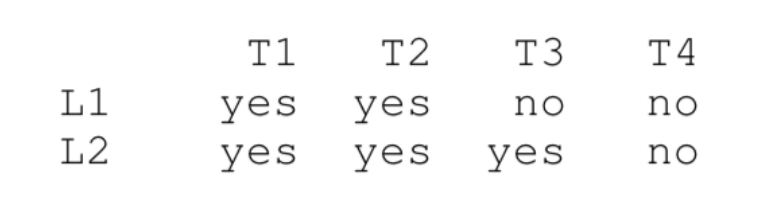
\includegraphics[width=0.3\textwidth]{chapters/Cucurrency/Cucurrency/schedule_avoid_1.png}

    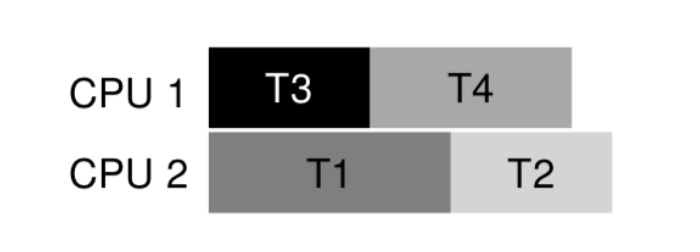
\includegraphics[width=0.3\textwidth]{chapters/Cucurrency/Cucurrency/good_schedule_1.png}


    From the images, it is possible to schedule threads to avoid deadlock\\
    \underline{\textbf{ if we need the resources that eac thread wants before hand}}.

    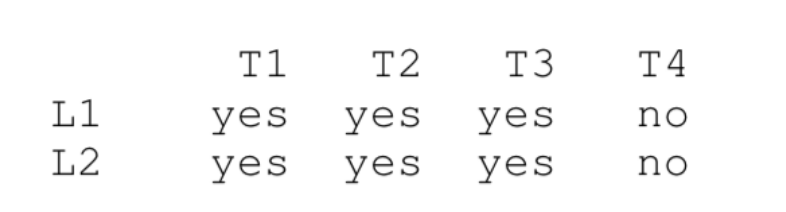
\includegraphics[width=0.3\textwidth]{chapters/Cucurrency/Cucurrency/deadlock_avoid_2.png}

    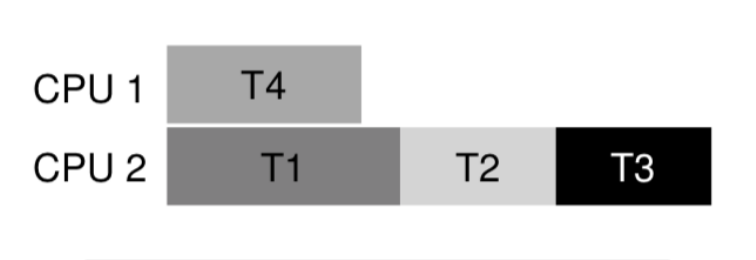
\includegraphics[width=0.3\textwidth]{chapters/Cucurrency/Cucurrency/schedule_2.png}

    Also, the scheduler could procude length-considerable scheduling.

    Thus, this approach can be only used in limited environment, for example,
    in an embedded system where one has full knowledge of the entire
    set of tasks must be run and the locks that they need.

    Also, such approach can limit the degree of concurrency.

\sssc{Detection And Recovery}

    One strategy can allow deadlock to occur occasionally, and then take some 
    action once it has been detected.

    A deadlock detector runs periodically,
     building a resource graph and checking it for cycles.